\makeatletter \@ifundefined{rootpath}{% Manual to memoir http://mirrors.dotsrc.org/ctan/macros/latex/contrib/memoir/memman.pdf

%\documentclass[a4paper,12pt,fleqn,openany,twoside]{memoir} %two sides for printing
\documentclass[a4paper,12pt,fleqn,openany,oneside]{memoir} %one side for pdf
\usepackage[english]{babel}
\usepackage[utf8]{inputenc}
\usepackage{microtype}
\usepackage{paralist}

%Definitions
\usepackage{amsthm}
\theoremstyle{plain}
\newtheorem{thm}{Theorem}[chapter] % reset theorem numbering for each chapter
\theoremstyle{definition}
\newtheorem{defn}[thm]{Definition}

% Choses the depth of numerations
\setsecnumdepth{subsubsection}

% Choses the depth of toc
%\maxtocdepth{subsection}

% Turn figures sideways with \begin{sideways} figure \end{sideways}
\usepackage{rotating}

% LaTeX logical statements
\usepackage{ifthen}

% Fancy space after use of e.g. command
\usepackage{xspace}

% Skips after paragraphs
\usepackage{parskip}

% Layout settings
\setlength{\parindent}{0cm}
\setlength{\parskip}{2ex plus 2ex} %kan udvides til f.eks: '2ex plus 2ex minus 0ex'

\sloppybottom

% Don't make a collection per default
\newcommand{\worksheetcollection}{false}

% Bibtex
\usepackage[square,numbers,sort,comma]{natbib}
%\usepackage{cite}
%\bibliographystyle{plainnat}
\bibliographystyle{IEEEtran}


% Fixmes
\usepackage{fixme}
\fxsetup{draft}

% Mathematic
\usepackage{amsmath}
\usepackage{amsfonts}
\usepackage{amssymb}
\usepackage{stmaryrd}
\allowdisplaybreaks[1]


% Acronyms
\usepackage[printonlyused]{acronym}

% Images
\usepackage{graphicx}
\usepackage{wrapfig}
\usepackage[outdir=./]{epstopdf}
\usepackage{epsfig}


% Captions ans subcaptions
\captionnamefont{\footnotesize\bfseries}
\captiontitlefont{\footnotesize}

% Enable memoir subfloats for figures and tables
\newsubfloat{figure}
\newsubfloat{table}

% Hack memoir subfigure styles to have bold label and footnotesize fonts
\renewcommand{\thesubfigure}{\footnotesize\bfseries{(\alph{subfigure})}}
\renewcommand{\thesubtable}{\footnotesize\bfseries{(\alph{subtable})}}

\renewcommand{\subcaption}[2][]{\subbottom[\footnotesize{#1}]{#2}}

% Memoir tweak pagenumbers
%\pagestyle{headings}

% Tikz
\usepackage{tikz}
\usetikzlibrary{arrows,shapes,calc,positioning}
\pgfmathsetseed{1}

%Pgf plots
\usepackage{pgfplots}
\pgfplotsset{compat=1.5}
% loatbarrier, keep figures within (sub,subsub) sections
\usepackage{placeins}
\usepackage{pgfplots}
\usepgfplotslibrary{units}
\usepackage[space-before-unit,range-units = repeat]{siunitx}

% Hyperlinked auto references
\usepackage[hidelinks]{hyperref}
\usepackage[nameinlink]{cleveref}
\crefname{lstlisting}{Listing}{Listings}  
\Crefname{lstlisting}{Listing}{Listings}

\crefname{thm}{definition}{definitions}
\Crefname{thm}{Definition}{Definitions}

%\def\chapterautorefname{Kapitel}
%\def\sectionautorefname{Afsnit}
%\def\subsectionautorefname{Afsnit}
%\def\subsubsectionautorefname{Underafsnit}
%\def\figureautorefname{Figur}
%\def\lstlistingautorefname{Listing}
%\def\lstnumberautorefname{Linje}
%\def\itemautorefname{Punkt}
\usepackage[hypcap]{caption} % Link to top of the figure and not the caption

%Sick shit to make \Autoref command
%http://tex.stackexchange.com/questions/36575/autorefs-inserted-text-has-not-the-correct-case
\def\HyLang@english{%
  \def\equationautorefname{Equation}%
  \def\footnoteautorefname{Footnote}%
  \def\itemautorefname{item}%
  \def\figureautorefname{Figure}%
  \def\tableautorefname{Table}%
  \def\partautorefname{Part}%
  \def\appendixautorefname{Appendix}%
  \def\chapterautorefname{Chapter}%
  \def\sectionautorefname{Section}%
  \def\subsectionautorefname{Subsection}%
  \def\subsubsectionautorefname{Subsubsection}%
  \def\paragraphautorefname{Paragraph}%
  \def\subparagraphautorefname{Subparagraph}%
  \def\FancyVerbLineautorefname{Line}%
  \def\theoremautorefname{Theorem}%
  \def\pageautorefname{Page}%
}

% Reference greencommentssections with number and name
\usepackage{nameref}
\newcommand{\bsnameref}[1]{\Cref{#1} ``\nameref{#1}''}
\newcommand{\bsref}[1]{\Cref{#1}}
\newcommand{\bsbilagref}[1]{Appendix \ref{#1}}
\newcommand{\bsbilagnameref}[1]{Appendix \ref{#1} ``\nameref{#1}''}
\newcommand{\pling}[1]{``#1''}


% Listings for code qoutes
\usepackage{listings}
%\usepackage[usenames,dvipsnames,svgnames,table]{xcolor}
\usepackage{color}
\usepackage{xcolor}
\definecolor{bluekeywords}{rgb}{0.13,0.13,1}
\definecolor{greencomments}{rgb}{0,0.5,0}
\definecolor{redstrings}{rgb}{0.9,0,0}
\usepackage{caption} 
\usepackage{multicol}
\DeclareCaptionFont{white}{\color{white}}
\DeclareCaptionFormat{listing}{\colorbox{gray}{\parbox{\textwidth}{#1#2#3}}}
\captionsetup[lstlisting]{format=listing,labelfont=white,textfont=white}
%\lstset{numbers=left}
\usepackage{courier}
\lstset{
	basicstyle=\footnotesize\ttfamily,
	tabsize=2,
	breaklines=true,
  literate={æ}{{\ae}}1 {ø}{{\o}}1 {å}{{\aa}}1 {Æ}{{\AE}}1 {Ø}{{\O}}1 {Å}{{\AA}}1,
  keywords={typeof, new, true, false, catch, function, return, null, catch, switch, var, if, in, while, do, else, case, break},
  keywordstyle=\color{blue}\bfseries,
  ndkeywords={class, export, boolean, throw, implements, import, using, this},
  ndkeywordstyle=\color{darkgray}\bfseries,
  identifierstyle=\color{black},
  sensitive=false,
  comment=[l]{//},
  morecomment=[s]{/*}{*/},
  commentstyle=\color{purple}\ttfamily,
  stringstyle=\color{red}\ttfamily,
  numbers=left,
  numbersep=-5pt,
  showstringspaces=false,
  showspaces=false,
  %morestring=[b]',
  %morestring=[b]"
}
\lstnewenvironment{code}[1][]%
  {\minipage{\linewidth} 
   \lstset{basicstyle=\ttfamily\footnotesize,frame=single,#1}}
  {\endminipage}

\lstdefinelanguage{scala}{
  morekeywords={abstract,case,catch,class,def,%
    do,else,extends,false,final,finally,%
    for,if,implicit,import,match,mixin,%
    new,null,object,override,package,%
    private,protected,requires,return,sealed,%
    super,this,throw,trait,true,try,%
    type,val,var,while,with,yield, Unit, Boolean, Int},
  otherkeywords={=>,<-,<\%,<:,>:,\#,@},
  sensitive=true,
  morecomment=[l]{//},
  morecomment=[n]{/*}{*/},
  morestring=[b]",
  morestring=[b]',
  morestring=[b]"""
}

\lstdefinelanguage{clojure}%
{morekeywords={*,*1,*2,*3,*agent*,*allow-unresolved-vars*,*assert*,*clojure-version*,*command-line-args*,%
*compile-files*,*compile-path*,*e,*err*,*file*,*flush-on-newline*,*in*,*macro-meta*,%
*math-context*,*ns*,*out*,*print-dup*,*print-length*,*print-level*,*print-meta*,*print-readably*,%
*read-eval*,*source-path*,*use-context-classloader*,*warn-on-reflection*,+,-,->,->>,..,/,:else,%
<,<=,=,==,>,>=,@,accessor,aclone,add-classpath,add-watch,agent,agent-errors,aget,alength,alias,%
all-ns,alter,alter-meta!,alter-var-root,amap,ancestors,and,apply,areduce,array-map,aset,%
aset-boolean,aset-byte,aset-char,aset-double,aset-float,aset-int,aset-long,aset-short,assert,%
assoc,assoc!,assoc-in,associative?,atom,await,await-for,await1,bases,bean,bigdec,bigint,binding,%
bit-and,bit-and-not,bit-clear,bit-flip,bit-not,bit-or,bit-set,bit-shift-left,bit-shift-right,%
bit-test,bit-xor,boolean,boolean-array,booleans,bound-fn,bound-fn*,butlast,byte,byte-array,%
bytes,cast,char,char-array,char-escape-string,char-name-string,char?,chars,chunk,chunk-append,%
chunk-buffer,chunk-cons,chunk-first,chunk-next,chunk-rest,chunked-seq?,class,class?,%
clear-agent-errors,clojure-version,coll?,comment,commute,comp,comparator,compare,compare-and-set!,%
compile,complement,concat,cond,condp,conj,conj!,cons,constantly,construct-proxy,contains?,count,%
counted?,create-ns,create-struct,cycle,dec,decimal?,declare,def,definline,defmacro,defmethod,%
defmulti,defn,defn-,defonce,defprotocol,defstruct,deftype,delay,delay?,deliver,deref,derive,%
descendants,destructure,disj,disj!,dissoc,dissoc!,distinct,distinct?,do,do-template,doall,doc,%
dorun,doseq,dosync,dotimes,doto,double,double-array,doubles,drop,drop-last,drop-while,empty,empty?,%
ensure,enumeration-seq,eval,even?,every?,false,false?,ffirst,file-seq,filter,finally,find,find-doc,%
find-ns,find-var,first,float,float-array,float?,floats,flush,fn,fn?,fnext,for,force,format,future,%
future-call,future-cancel,future-cancelled?,future-done?,future?,gen-class,gen-interface,gensym,%
get,get-in,get-method,get-proxy-class,get-thread-bindings,get-validator,hash,hash-map,hash-set,%
identical?,identity,if,if-let,if-not,ifn?,import,in-ns,inc,init-proxy,instance?,int,int-array,%
integer?,interleave,intern,interpose,into,into-array,ints,io!,isa?,iterate,iterator-seq,juxt,%
key,keys,keyword,keyword?,last,lazy-cat,lazy-seq,let,letfn,line-seq,list,list*,list?,load,load-file,%
load-reader,load-string,loaded-libs,locking,long,long-array,longs,loop,macroexpand,macroexpand-1,%
make-array,make-hierarchy,map,map?,mapcat,max,max-key,memfn,memoize,merge,merge-with,meta,%
method-sig,methods,min,min-key,mod,monitor-enter,monitor-exit,name,namespace,neg?,new,newline,%
next,nfirst,nil,nil?,nnext,not,not-any?,not-empty,not-every?,not=,ns,ns-aliases,ns-imports,%
ns-interns,ns-map,ns-name,ns-publics,ns-refers,ns-resolve,ns-unalias,ns-unmap,nth,nthnext,num,%
number?,odd?,or,parents,partial,partition,pcalls,peek,persistent!,pmap,pop,pop!,pop-thread-bindings,%
pos?,pr,pr-str,prefer-method,prefers,primitives-classnames,print,print-ctor,print-doc,print-dup,%
print-method,print-namespace-doc,print-simple,print-special-doc,print-str,printf,println,println-str,%
prn,prn-str,promise,proxy,proxy-call-with-super,proxy-mappings,proxy-name,proxy-super,%
push-thread-bindings,pvalues,quot,rand,rand-int,range,ratio?,rational?,rationalize,re-find,%
re-groups,re-matcher,re-matches,re-pattern,re-seq,read,read-line,read-string,recur,reduce,ref,%
ref-history-count,ref-max-history,ref-min-history,ref-set,refer,refer-clojure,reify,%
release-pending-sends,rem,remove,remove-method,remove-ns,remove-watch,repeat,repeatedly,%
replace,replicate,require,reset!,reset-meta!,resolve,rest,resultset-seq,reverse,reversible?,%
rseq,rsubseq,second,select-keys,send,send-off,seq,seq?,seque,sequence,sequential?,set,set!,%
set-validator!,set?,short,short-array,shorts,shutdown-agents,slurp,some,sort,sort-by,sorted-map,%
sorted-map-by,sorted-set,sorted-set-by,sorted?,special-form-anchor,special-symbol?,split-at,%
split-with,str,stream?,string?,struct,struct-map,subs,subseq,subvec,supers,swap!,symbol,symbol?,%
sync,syntax-symbol-anchor,take,take-last,take-nth,take-while,test,the-ns,throw,time,to-array,%
to-array-2d,trampoline,transient,tree-seq,true,true?,try,type,unchecked-add,unchecked-dec,%
unchecked-divide,unchecked-inc,unchecked-multiply,unchecked-negate,unchecked-remainder,%
unchecked-subtract,underive,unquote,unquote-splicing,update-in,update-proxy,use,val,vals,%
var,var-get,var-set,var?,vary-meta,vec,vector,vector?,when,when-first,when-let,when-not,%
while,with-bindings,with-bindings*,with-in-str,with-loading-context,with-local-vars,%
with-meta,with-open,with-out-str,with-precision,xml-seq,zero?,zipmap
},%
   sensitive,% ???
   alsodigit=-,%
   morecomment=[l];,%
   morestring=[b]"%
  }[keywords,comments,strings]%

% Worksheet commands
\newcommand{\worksheetstart}[5]{ %Title, Revision, Date, Author, rootpath
	\ifthenelse{\equal{\worksheetcollection}{false}}{
		\newcommand{\rootpath}{#5}
		\documentheader
		\chapter{#1}
	}{
		\chapter{#1}
	}
%	\vspace{-1em}
%	\textbf{\tiny Revision #2 at #3. Written by #4}\\
%	\textbf{\tiny Hovedansvarlig #4}\\
%	\vspace{2em}\\
}

\newcommand{\worksheetend}{
	\ifthenelse{\equal{\worksheetcollection}{false}}{
		\collectionend
	}{}
}

\newcommand{\documentheader}{
	% Draws a tikz camera
% #1 is the coordinate to the top left corner
% #2 is a label for the righthand center position
% #3 is the text shown in the center of the camera
\newcommand{\camera}[3]{
\coordinate (anchor) at #1;
\draw (anchor) -- ($ (anchor) + (0em,-20pt) $) -- ($ (anchor) + (10pt, -15pt) $) -- ($ (anchor) + (10pt,-5pt)$) -- cycle;
\draw ($ (anchor) + (10pt,-5pt) $) -- ($ (anchor) + (10pt,0pt) $) -- ($ (anchor) + (50pt,0pt) $) -- ($ (anchor) + (50pt,-20pt) $) -- node[yshift=10pt] {\tiny #3} ($ (anchor) + (10pt,-20pt) $)-- cycle;
\coordinate (#2) at ($ (anchor) + (50pt,-10pt) $);
}

\newcounter{frameNumber}
\newcommand{\frameWithSize}[3][false]{
	\stepcounter{frameNumber}
	\coordinate (anchor) at #2;
	\ifthenelse{\equal{#1}{false}}{
		\def\frameNumber{\arabic{frameNumber}}
	}{
		\def\frameNumber{#1}
	}
	\pgfmathtruncatemacro\randomnumber{random(0,4)}
	\node[yshift=20pt] at (anchor) {\frameNumber};
	\ifthenelse{\equal{#3}{I}}{
		\node[draw, minimum size=20pt, fill=green!60] at (anchor) {I};
		\filldraw[fill=gray] ($(anchor) + (-10pt,-40pt)$) rectangle ($(anchor) + (10pt,-20pt) + (0pt,\randomnumber pt)$);
	}{
		\ifthenelse{\equal{#3}{P}}{
			\node[draw, minimum size=20pt, fill=yellow!60] at (anchor) {P};
			\filldraw[fill=gray] ($(anchor) + (-10pt,-40pt)$) rectangle ($(anchor) + (10pt,-30pt) + (0pt,\randomnumber pt)$);
		}{
			\node[draw, minimum size=20pt, fill=blue!40!yellow!60!black] at (anchor) {\color{white}B};
			\filldraw[fill=gray] ($(anchor) + (-10pt,-40pt)$) rectangle ($(anchor) + (10pt,-37pt) + (0pt,\randomnumber pt)$);
		}
	}
	\draw[thick] ($(anchor) + (-10pt,-40pt)$) -- +(20pt,0pt);
}

	\begin{document}
	%\renewcommand{\chaptername}{Worksheet}
	\chapterstyle{section}
	\renewcommand{\beforechapskip}{0pt}
	\renewcommand{\afterchapskip}{0pt}
}

\newcommand{\collectionstart}[1]{
	\newcommand{\rootpath}{#1}
	\renewcommand{\worksheetcollection}{true}
	\documentheader
	\frontmatter
	%\forside
	\makeatletter \@ifundefined{rootpath}{% Manual to memoir http://mirrors.dotsrc.org/ctan/macros/latex/contrib/memoir/memman.pdf

%\documentclass[a4paper,12pt,fleqn,openany,twoside]{memoir} %two sides for printing
\documentclass[a4paper,12pt,fleqn,openany,oneside]{memoir} %one side for pdf
\usepackage[english]{babel}
\usepackage[utf8]{inputenc}
\usepackage{microtype}
\usepackage{paralist}

%Definitions
\usepackage{amsthm}
\theoremstyle{plain}
\newtheorem{thm}{Theorem}[chapter] % reset theorem numbering for each chapter
\theoremstyle{definition}
\newtheorem{defn}[thm]{Definition}

% Choses the depth of numerations
\setsecnumdepth{subsubsection}

% Choses the depth of toc
%\maxtocdepth{subsection}

% Turn figures sideways with \begin{sideways} figure \end{sideways}
\usepackage{rotating}

% LaTeX logical statements
\usepackage{ifthen}

% Fancy space after use of e.g. command
\usepackage{xspace}

% Skips after paragraphs
\usepackage{parskip}

% Layout settings
\setlength{\parindent}{0cm}
\setlength{\parskip}{2ex plus 2ex} %kan udvides til f.eks: '2ex plus 2ex minus 0ex'

\sloppybottom

% Don't make a collection per default
\newcommand{\worksheetcollection}{false}

% Bibtex
\usepackage[square,numbers,sort,comma]{natbib}
%\usepackage{cite}
%\bibliographystyle{plainnat}
\bibliographystyle{IEEEtran}


% Fixmes
\usepackage{fixme}
\fxsetup{draft}

% Mathematic
\usepackage{amsmath}
\usepackage{amsfonts}
\usepackage{amssymb}
\usepackage{stmaryrd}
\allowdisplaybreaks[1]


% Acronyms
\usepackage[printonlyused]{acronym}

% Images
\usepackage{graphicx}
\usepackage{wrapfig}
\usepackage[outdir=./]{epstopdf}
\usepackage{epsfig}


% Captions ans subcaptions
\captionnamefont{\footnotesize\bfseries}
\captiontitlefont{\footnotesize}

% Enable memoir subfloats for figures and tables
\newsubfloat{figure}
\newsubfloat{table}

% Hack memoir subfigure styles to have bold label and footnotesize fonts
\renewcommand{\thesubfigure}{\footnotesize\bfseries{(\alph{subfigure})}}
\renewcommand{\thesubtable}{\footnotesize\bfseries{(\alph{subtable})}}

\renewcommand{\subcaption}[2][]{\subbottom[\footnotesize{#1}]{#2}}

% Memoir tweak pagenumbers
%\pagestyle{headings}

% Tikz
\usepackage{tikz}
\usetikzlibrary{arrows,shapes,calc,positioning}
\pgfmathsetseed{1}

%Pgf plots
\usepackage{pgfplots}
\pgfplotsset{compat=1.5}
% loatbarrier, keep figures within (sub,subsub) sections
\usepackage{placeins}
\usepackage{pgfplots}
\usepgfplotslibrary{units}
\usepackage[space-before-unit,range-units = repeat]{siunitx}

% Hyperlinked auto references
\usepackage[hidelinks]{hyperref}
\usepackage[nameinlink]{cleveref}
\crefname{lstlisting}{Listing}{Listings}  
\Crefname{lstlisting}{Listing}{Listings}

\crefname{thm}{definition}{definitions}
\Crefname{thm}{Definition}{Definitions}

%\def\chapterautorefname{Kapitel}
%\def\sectionautorefname{Afsnit}
%\def\subsectionautorefname{Afsnit}
%\def\subsubsectionautorefname{Underafsnit}
%\def\figureautorefname{Figur}
%\def\lstlistingautorefname{Listing}
%\def\lstnumberautorefname{Linje}
%\def\itemautorefname{Punkt}
\usepackage[hypcap]{caption} % Link to top of the figure and not the caption

%Sick shit to make \Autoref command
%http://tex.stackexchange.com/questions/36575/autorefs-inserted-text-has-not-the-correct-case
\def\HyLang@english{%
  \def\equationautorefname{Equation}%
  \def\footnoteautorefname{Footnote}%
  \def\itemautorefname{item}%
  \def\figureautorefname{Figure}%
  \def\tableautorefname{Table}%
  \def\partautorefname{Part}%
  \def\appendixautorefname{Appendix}%
  \def\chapterautorefname{Chapter}%
  \def\sectionautorefname{Section}%
  \def\subsectionautorefname{Subsection}%
  \def\subsubsectionautorefname{Subsubsection}%
  \def\paragraphautorefname{Paragraph}%
  \def\subparagraphautorefname{Subparagraph}%
  \def\FancyVerbLineautorefname{Line}%
  \def\theoremautorefname{Theorem}%
  \def\pageautorefname{Page}%
}

% Reference greencommentssections with number and name
\usepackage{nameref}
\newcommand{\bsnameref}[1]{\Cref{#1} ``\nameref{#1}''}
\newcommand{\bsref}[1]{\Cref{#1}}
\newcommand{\bsbilagref}[1]{Appendix \ref{#1}}
\newcommand{\bsbilagnameref}[1]{Appendix \ref{#1} ``\nameref{#1}''}
\newcommand{\pling}[1]{``#1''}


% Listings for code qoutes
\usepackage{listings}
%\usepackage[usenames,dvipsnames,svgnames,table]{xcolor}
\usepackage{color}
\usepackage{xcolor}
\definecolor{bluekeywords}{rgb}{0.13,0.13,1}
\definecolor{greencomments}{rgb}{0,0.5,0}
\definecolor{redstrings}{rgb}{0.9,0,0}
\usepackage{caption} 
\usepackage{multicol}
\DeclareCaptionFont{white}{\color{white}}
\DeclareCaptionFormat{listing}{\colorbox{gray}{\parbox{\textwidth}{#1#2#3}}}
\captionsetup[lstlisting]{format=listing,labelfont=white,textfont=white}
%\lstset{numbers=left}
\usepackage{courier}
\lstset{
	basicstyle=\footnotesize\ttfamily,
	tabsize=2,
	breaklines=true,
  literate={æ}{{\ae}}1 {ø}{{\o}}1 {å}{{\aa}}1 {Æ}{{\AE}}1 {Ø}{{\O}}1 {Å}{{\AA}}1,
  keywords={typeof, new, true, false, catch, function, return, null, catch, switch, var, if, in, while, do, else, case, break},
  keywordstyle=\color{blue}\bfseries,
  ndkeywords={class, export, boolean, throw, implements, import, using, this},
  ndkeywordstyle=\color{darkgray}\bfseries,
  identifierstyle=\color{black},
  sensitive=false,
  comment=[l]{//},
  morecomment=[s]{/*}{*/},
  commentstyle=\color{purple}\ttfamily,
  stringstyle=\color{red}\ttfamily,
  numbers=left,
  numbersep=-5pt,
  showstringspaces=false,
  showspaces=false,
  %morestring=[b]',
  %morestring=[b]"
}
\lstnewenvironment{code}[1][]%
  {\minipage{\linewidth} 
   \lstset{basicstyle=\ttfamily\footnotesize,frame=single,#1}}
  {\endminipage}

\lstdefinelanguage{scala}{
  morekeywords={abstract,case,catch,class,def,%
    do,else,extends,false,final,finally,%
    for,if,implicit,import,match,mixin,%
    new,null,object,override,package,%
    private,protected,requires,return,sealed,%
    super,this,throw,trait,true,try,%
    type,val,var,while,with,yield, Unit, Boolean, Int},
  otherkeywords={=>,<-,<\%,<:,>:,\#,@},
  sensitive=true,
  morecomment=[l]{//},
  morecomment=[n]{/*}{*/},
  morestring=[b]",
  morestring=[b]',
  morestring=[b]"""
}

\lstdefinelanguage{clojure}%
{morekeywords={*,*1,*2,*3,*agent*,*allow-unresolved-vars*,*assert*,*clojure-version*,*command-line-args*,%
*compile-files*,*compile-path*,*e,*err*,*file*,*flush-on-newline*,*in*,*macro-meta*,%
*math-context*,*ns*,*out*,*print-dup*,*print-length*,*print-level*,*print-meta*,*print-readably*,%
*read-eval*,*source-path*,*use-context-classloader*,*warn-on-reflection*,+,-,->,->>,..,/,:else,%
<,<=,=,==,>,>=,@,accessor,aclone,add-classpath,add-watch,agent,agent-errors,aget,alength,alias,%
all-ns,alter,alter-meta!,alter-var-root,amap,ancestors,and,apply,areduce,array-map,aset,%
aset-boolean,aset-byte,aset-char,aset-double,aset-float,aset-int,aset-long,aset-short,assert,%
assoc,assoc!,assoc-in,associative?,atom,await,await-for,await1,bases,bean,bigdec,bigint,binding,%
bit-and,bit-and-not,bit-clear,bit-flip,bit-not,bit-or,bit-set,bit-shift-left,bit-shift-right,%
bit-test,bit-xor,boolean,boolean-array,booleans,bound-fn,bound-fn*,butlast,byte,byte-array,%
bytes,cast,char,char-array,char-escape-string,char-name-string,char?,chars,chunk,chunk-append,%
chunk-buffer,chunk-cons,chunk-first,chunk-next,chunk-rest,chunked-seq?,class,class?,%
clear-agent-errors,clojure-version,coll?,comment,commute,comp,comparator,compare,compare-and-set!,%
compile,complement,concat,cond,condp,conj,conj!,cons,constantly,construct-proxy,contains?,count,%
counted?,create-ns,create-struct,cycle,dec,decimal?,declare,def,definline,defmacro,defmethod,%
defmulti,defn,defn-,defonce,defprotocol,defstruct,deftype,delay,delay?,deliver,deref,derive,%
descendants,destructure,disj,disj!,dissoc,dissoc!,distinct,distinct?,do,do-template,doall,doc,%
dorun,doseq,dosync,dotimes,doto,double,double-array,doubles,drop,drop-last,drop-while,empty,empty?,%
ensure,enumeration-seq,eval,even?,every?,false,false?,ffirst,file-seq,filter,finally,find,find-doc,%
find-ns,find-var,first,float,float-array,float?,floats,flush,fn,fn?,fnext,for,force,format,future,%
future-call,future-cancel,future-cancelled?,future-done?,future?,gen-class,gen-interface,gensym,%
get,get-in,get-method,get-proxy-class,get-thread-bindings,get-validator,hash,hash-map,hash-set,%
identical?,identity,if,if-let,if-not,ifn?,import,in-ns,inc,init-proxy,instance?,int,int-array,%
integer?,interleave,intern,interpose,into,into-array,ints,io!,isa?,iterate,iterator-seq,juxt,%
key,keys,keyword,keyword?,last,lazy-cat,lazy-seq,let,letfn,line-seq,list,list*,list?,load,load-file,%
load-reader,load-string,loaded-libs,locking,long,long-array,longs,loop,macroexpand,macroexpand-1,%
make-array,make-hierarchy,map,map?,mapcat,max,max-key,memfn,memoize,merge,merge-with,meta,%
method-sig,methods,min,min-key,mod,monitor-enter,monitor-exit,name,namespace,neg?,new,newline,%
next,nfirst,nil,nil?,nnext,not,not-any?,not-empty,not-every?,not=,ns,ns-aliases,ns-imports,%
ns-interns,ns-map,ns-name,ns-publics,ns-refers,ns-resolve,ns-unalias,ns-unmap,nth,nthnext,num,%
number?,odd?,or,parents,partial,partition,pcalls,peek,persistent!,pmap,pop,pop!,pop-thread-bindings,%
pos?,pr,pr-str,prefer-method,prefers,primitives-classnames,print,print-ctor,print-doc,print-dup,%
print-method,print-namespace-doc,print-simple,print-special-doc,print-str,printf,println,println-str,%
prn,prn-str,promise,proxy,proxy-call-with-super,proxy-mappings,proxy-name,proxy-super,%
push-thread-bindings,pvalues,quot,rand,rand-int,range,ratio?,rational?,rationalize,re-find,%
re-groups,re-matcher,re-matches,re-pattern,re-seq,read,read-line,read-string,recur,reduce,ref,%
ref-history-count,ref-max-history,ref-min-history,ref-set,refer,refer-clojure,reify,%
release-pending-sends,rem,remove,remove-method,remove-ns,remove-watch,repeat,repeatedly,%
replace,replicate,require,reset!,reset-meta!,resolve,rest,resultset-seq,reverse,reversible?,%
rseq,rsubseq,second,select-keys,send,send-off,seq,seq?,seque,sequence,sequential?,set,set!,%
set-validator!,set?,short,short-array,shorts,shutdown-agents,slurp,some,sort,sort-by,sorted-map,%
sorted-map-by,sorted-set,sorted-set-by,sorted?,special-form-anchor,special-symbol?,split-at,%
split-with,str,stream?,string?,struct,struct-map,subs,subseq,subvec,supers,swap!,symbol,symbol?,%
sync,syntax-symbol-anchor,take,take-last,take-nth,take-while,test,the-ns,throw,time,to-array,%
to-array-2d,trampoline,transient,tree-seq,true,true?,try,type,unchecked-add,unchecked-dec,%
unchecked-divide,unchecked-inc,unchecked-multiply,unchecked-negate,unchecked-remainder,%
unchecked-subtract,underive,unquote,unquote-splicing,update-in,update-proxy,use,val,vals,%
var,var-get,var-set,var?,vary-meta,vec,vector,vector?,when,when-first,when-let,when-not,%
while,with-bindings,with-bindings*,with-in-str,with-loading-context,with-local-vars,%
with-meta,with-open,with-out-str,with-precision,xml-seq,zero?,zipmap
},%
   sensitive,% ???
   alsodigit=-,%
   morecomment=[l];,%
   morestring=[b]"%
  }[keywords,comments,strings]%

% Worksheet commands
\newcommand{\worksheetstart}[5]{ %Title, Revision, Date, Author, rootpath
	\ifthenelse{\equal{\worksheetcollection}{false}}{
		\newcommand{\rootpath}{#5}
		\documentheader
		\chapter{#1}
	}{
		\chapter{#1}
	}
%	\vspace{-1em}
%	\textbf{\tiny Revision #2 at #3. Written by #4}\\
%	\textbf{\tiny Hovedansvarlig #4}\\
%	\vspace{2em}\\
}

\newcommand{\worksheetend}{
	\ifthenelse{\equal{\worksheetcollection}{false}}{
		\collectionend
	}{}
}

\newcommand{\documentheader}{
	\input{\rootpath/setup/tikz-commands.tex}
	\begin{document}
	%\renewcommand{\chaptername}{Worksheet}
	\chapterstyle{section}
	\renewcommand{\beforechapskip}{0pt}
	\renewcommand{\afterchapskip}{0pt}
}

\newcommand{\collectionstart}[1]{
	\newcommand{\rootpath}{#1}
	\renewcommand{\worksheetcollection}{true}
	\documentheader
	\frontmatter
	%\forside
	\input{\rootpath/worksheets/titlepage/titlepage}
	\input{\rootpath/worksheets/preface/preface}
	%\input{\rootpath/worksheets/forord/forord}
	\newpage
	\newpage
	\tableofcontents*
	\mainmatter
}

\newcommand{\collectionend}{
	\backmatter
	\chapter{List of Acronyms}\vspace{3em}
	\input{\rootpath/setup/acronyms}
	\bibliography{\rootpath/setup/bibliography}
	\end{document}
}


%\newcommand{\bscode}{
%	\lstinline
%}

\font\fontcode=pcrr at 12pt

\newcommand{\bscode}[1]{
	{\fontcode#1}
}



\newcommand{\bscodemath}[1]{
	\text{\lstinline|#1|}
}

\newcommand{\bsqoute}[2]{
	\begin{quote}
		\textit{``#1''}
		\begin{center}
			-- \emph{#2}
		\end{center}
	\end{quote}
}


\newcommand{\lag}{\langle}
\newcommand{\rag}{\rangle}
\newcommand{\besk}[1]{\ensuremath{\lag #1 \rag}}

\newcommand{\namedtodo}[5]
{
  \ifthenelse{\equal{#1}{}}
  {
    \todo[color=#4,caption=
    {\textbf{#3: } #2}]
    {\color{#5}\textbf{#3: }#2}
  }
  {
    \todo[color=#4,caption=
    {\textbf{#3: } #1}
    ,inline]
    {\color{#5}\textbf{#3: }#2}
  }
}
\newcommand{\andreas}[2][]{\namedtodo{#1}{#2}{Andreas}{blue!50!red!10}{black}}
\newcommand{\lone}[2][]{\namedtodo{#1}{#2}{Lone}{orange}{black}}
\definecolor{babypink}{rgb}{0.96, 0.76, 0.76}
\newcommand{\toby}[2][]{\namedtodo{#1}{#2}{Tobias}{babypink}{black}}
\newcommand{\kasper}[2][]{\namedtodo{#1}{#2}{Kasper}{green}{black}}

%multicol
\usepackage{multicol}

% todonotes
%\usepackage[disable]{todonotes} %For final report
\usepackage{todonotes} %For writing notes
\usepackage{fancyvrb}

%Loading AAU macro
\usepackage{lastpage}
%%%%%%%%%%%%%%%%%%%%%%%%%%%%%%%%%%%%%%%%%%%%%%%%
% Macros for the titlepage
%%%%%%%%%%%%%%%%%%%%%%%%%%%%%%%%%%%%%%%%%%%%%%%%
%Creates the aau titlepage
\newcommand{\aautitlepage}[3]{%
  {
    %set up various length
    \ifx\titlepageleftcolumnwidth\undefined
      \newlength{\titlepageleftcolumnwidth}
      \newlength{\titlepagerightcolumnwidth}
    \fi
    \setlength{\titlepageleftcolumnwidth}{0.5\textwidth-\tabcolsep}
    \setlength{\titlepagerightcolumnwidth}{\textwidth-2\tabcolsep-\titlepageleftcolumnwidth}
    %create title page
    \thispagestyle{empty}
    \noindent%
    \begin{tabular}{@{}ll@{}}
      \parbox{\titlepageleftcolumnwidth}{
        \iflanguage{danish}{%
          
\includegraphics[width=\titlepageleftcolumnwidth]{titlepage/figures/aau_logo_da}
        }{%
          
\includegraphics[width=\titlepageleftcolumnwidth]{titlepage/figures/aau_logo_en}
        }
      } &
      \parbox{\titlepagerightcolumnwidth}{\raggedleft\small
        #2
      }\bigskip\\
       #1 &
      \parbox[t]{\titlepagerightcolumnwidth}{%
      \textbf{Abstract:}\bigskip\par
        \fbox{\parbox{\titlepagerightcolumnwidth-2\fboxsep-2\fboxrule}{%
          #3
        }}
      }\\
    \end{tabular}
    \vfill  
    \clearpage
  }
}

% Environment for problem statements
% Can be auto referenced.
\newtheorem{problem}{Problem}
\def\problemautorefname{Problem}

%Create english project info
\newcommand{\englishprojectinfo}[6]{%
  \parbox[t]{\titlepageleftcolumnwidth}{
    \textbf{Title:}\\ #1\bigskip\par
    %\textbf{Theme:}\\ #2\bigskip\par
    \textbf{Project Period:}\\ #2\bigskip\par
    \textbf{Project Group:}\\ #3\bigskip\par
    \textbf{Participants:}\\ #4\bigskip\par
    \textbf{Supervisor:}\\ #5\bigskip\par
    %\textbf{Copies:} #6\bigskip\par
    \textbf{Page Numbers:} \pageref{LastPage}\bigskip\par
    \textbf{Date of Completion:}\\ #6
  }
}



%Create danish project info
%\newcommand{\danishprojectinfo}[7]{%
 % \parbox[t]{\titlepageleftcolumnwidth}{
 %   \textbf{Titel:}\\ #1\bigskip\par
%    %\textbf{Tema:}\\ #2\bigskip\par
%    \textbf{Projektperiode:}\\ #2\bigskip\par
%    \textbf{Projektgruppe:}\\ #4\bigskip\par
%    \textbf{Deltager(e):}\\ #5\bigskip\par
 %   \textbf{Vejleder(e):}\\ #6\bigskip\par
%    \textbf{Oplagstal:} #7\bigskip\par
   % \textbf{Sidetal:} \pageref{LastPage}\bigskip\par
  %  \textbf{Afleveringsdato:}\\ #8
 % }
%}


%roman numerals
%\newcommand*{\rom}[1]{\expandafter\@slowromancap\romannumeral #1@}
\newcommand{\rom}[1]{\uppercase\expandafter{\romannumeral #1\relax}}

%Hypothesis
\newtheorem{hypo}{Hypothesis}

%STM name
\newcommand{\stmname}{AtomiC\#}
\newcommand{\stmnamesp}{AtomiC\# }

}\makeatother
%\worksheetstart{Titlepage}{0}{December 31, 2012}{../../}
\begin{titlingpage}
\aautitlepage{%
  \englishprojectinfo{
    Language Integrated STM in C\# Using the Roslyn Compiler - An Alternative to Locking. %title
    %STM Integration in C\# and the Roslyn Compiler. %title
  }{%
    Spring Semester 2015 %project period
  }{%
    dpt109f15  % project group
  }{%
    %list of group members
    Tobias Ugleholdt Hansen\\
    Andreas Pørtner Karlsen\\ 
    Kasper Breinholt Laurberg\\
  }{%
    %list of supervisors
     Lone Leth Thomsen
  }{%
    \today % date of completion
  }%
}{%department and address
  \textbf{Department of Computer Science}\\
  Selma Lagerløfs Vej 300\\
  DK-9220 Aalborg Ø\\
  \href{http://www.cs.aau.dk}{http://www.cs.aau.dk}
}{% the abstract
% Our motivation
% What have we done
% How did we do it
% Our contribution
This master thesis investigates whether language integrated STM, in terms of usability, is a valid alternative to locking and provides additional benefits compared to library-based STM. In order to do so, an extension of C\# called \stmname has been implemented. \stmname extends C\# with language integrated support for STM, including conditional synchronization using the retry and orelse constructs as well as nesting of transactions.

\stmname was implemented by extending the open source Roslyn C\# compiler. To power \stmname a library-based STM system, based on the TL\rom{2} algorithm, was implemented. The extended Roslyn C\# compiler transforms \stmname source code to regular C\# code which utilizes the STM library. For each of the concurrency approaches: \stmname, library-based STM and locking in C\#, four different concurrency problems, representing different aspects of concurrent programming were implemented. These implementations were analyzed according to a set of usability characteristics facilitating a conclusion upon the usability of language integrated STM in the context of C\#. Our evaluation concludes that \stmname is a valid alternative to locking, and provides better usability than library based STM.}
\end{titlingpage}
	\makeatletter \@ifundefined{rootpath}{% Manual to memoir http://mirrors.dotsrc.org/ctan/macros/latex/contrib/memoir/memman.pdf

%\documentclass[a4paper,12pt,fleqn,openany,twoside]{memoir} %two sides for printing
\documentclass[a4paper,12pt,fleqn,openany,oneside]{memoir} %one side for pdf
\usepackage[english]{babel}
\usepackage[utf8]{inputenc}
\usepackage{microtype}
\usepackage{paralist}

%Definitions
\usepackage{amsthm}
\theoremstyle{plain}
\newtheorem{thm}{Theorem}[chapter] % reset theorem numbering for each chapter
\theoremstyle{definition}
\newtheorem{defn}[thm]{Definition}

% Choses the depth of numerations
\setsecnumdepth{subsubsection}

% Choses the depth of toc
%\maxtocdepth{subsection}

% Turn figures sideways with \begin{sideways} figure \end{sideways}
\usepackage{rotating}

% LaTeX logical statements
\usepackage{ifthen}

% Fancy space after use of e.g. command
\usepackage{xspace}

% Skips after paragraphs
\usepackage{parskip}

% Layout settings
\setlength{\parindent}{0cm}
\setlength{\parskip}{2ex plus 2ex} %kan udvides til f.eks: '2ex plus 2ex minus 0ex'

\sloppybottom

% Don't make a collection per default
\newcommand{\worksheetcollection}{false}

% Bibtex
\usepackage[square,numbers,sort,comma]{natbib}
%\usepackage{cite}
%\bibliographystyle{plainnat}
\bibliographystyle{IEEEtran}


% Fixmes
\usepackage{fixme}
\fxsetup{draft}

% Mathematic
\usepackage{amsmath}
\usepackage{amsfonts}
\usepackage{amssymb}
\usepackage{stmaryrd}
\allowdisplaybreaks[1]


% Acronyms
\usepackage[printonlyused]{acronym}

% Images
\usepackage{graphicx}
\usepackage{wrapfig}
\usepackage[outdir=./]{epstopdf}
\usepackage{epsfig}


% Captions ans subcaptions
\captionnamefont{\footnotesize\bfseries}
\captiontitlefont{\footnotesize}

% Enable memoir subfloats for figures and tables
\newsubfloat{figure}
\newsubfloat{table}

% Hack memoir subfigure styles to have bold label and footnotesize fonts
\renewcommand{\thesubfigure}{\footnotesize\bfseries{(\alph{subfigure})}}
\renewcommand{\thesubtable}{\footnotesize\bfseries{(\alph{subtable})}}

\renewcommand{\subcaption}[2][]{\subbottom[\footnotesize{#1}]{#2}}

% Memoir tweak pagenumbers
%\pagestyle{headings}

% Tikz
\usepackage{tikz}
\usetikzlibrary{arrows,shapes,calc,positioning}
\pgfmathsetseed{1}

%Pgf plots
\usepackage{pgfplots}
\pgfplotsset{compat=1.5}
% loatbarrier, keep figures within (sub,subsub) sections
\usepackage{placeins}
\usepackage{pgfplots}
\usepgfplotslibrary{units}
\usepackage[space-before-unit,range-units = repeat]{siunitx}

% Hyperlinked auto references
\usepackage[hidelinks]{hyperref}
\usepackage[nameinlink]{cleveref}
\crefname{lstlisting}{Listing}{Listings}  
\Crefname{lstlisting}{Listing}{Listings}

\crefname{thm}{definition}{definitions}
\Crefname{thm}{Definition}{Definitions}

%\def\chapterautorefname{Kapitel}
%\def\sectionautorefname{Afsnit}
%\def\subsectionautorefname{Afsnit}
%\def\subsubsectionautorefname{Underafsnit}
%\def\figureautorefname{Figur}
%\def\lstlistingautorefname{Listing}
%\def\lstnumberautorefname{Linje}
%\def\itemautorefname{Punkt}
\usepackage[hypcap]{caption} % Link to top of the figure and not the caption

%Sick shit to make \Autoref command
%http://tex.stackexchange.com/questions/36575/autorefs-inserted-text-has-not-the-correct-case
\def\HyLang@english{%
  \def\equationautorefname{Equation}%
  \def\footnoteautorefname{Footnote}%
  \def\itemautorefname{item}%
  \def\figureautorefname{Figure}%
  \def\tableautorefname{Table}%
  \def\partautorefname{Part}%
  \def\appendixautorefname{Appendix}%
  \def\chapterautorefname{Chapter}%
  \def\sectionautorefname{Section}%
  \def\subsectionautorefname{Subsection}%
  \def\subsubsectionautorefname{Subsubsection}%
  \def\paragraphautorefname{Paragraph}%
  \def\subparagraphautorefname{Subparagraph}%
  \def\FancyVerbLineautorefname{Line}%
  \def\theoremautorefname{Theorem}%
  \def\pageautorefname{Page}%
}

% Reference greencommentssections with number and name
\usepackage{nameref}
\newcommand{\bsnameref}[1]{\Cref{#1} ``\nameref{#1}''}
\newcommand{\bsref}[1]{\Cref{#1}}
\newcommand{\bsbilagref}[1]{Appendix \ref{#1}}
\newcommand{\bsbilagnameref}[1]{Appendix \ref{#1} ``\nameref{#1}''}
\newcommand{\pling}[1]{``#1''}


% Listings for code qoutes
\usepackage{listings}
%\usepackage[usenames,dvipsnames,svgnames,table]{xcolor}
\usepackage{color}
\usepackage{xcolor}
\definecolor{bluekeywords}{rgb}{0.13,0.13,1}
\definecolor{greencomments}{rgb}{0,0.5,0}
\definecolor{redstrings}{rgb}{0.9,0,0}
\usepackage{caption} 
\usepackage{multicol}
\DeclareCaptionFont{white}{\color{white}}
\DeclareCaptionFormat{listing}{\colorbox{gray}{\parbox{\textwidth}{#1#2#3}}}
\captionsetup[lstlisting]{format=listing,labelfont=white,textfont=white}
%\lstset{numbers=left}
\usepackage{courier}
\lstset{
	basicstyle=\footnotesize\ttfamily,
	tabsize=2,
	breaklines=true,
  literate={æ}{{\ae}}1 {ø}{{\o}}1 {å}{{\aa}}1 {Æ}{{\AE}}1 {Ø}{{\O}}1 {Å}{{\AA}}1,
  keywords={typeof, new, true, false, catch, function, return, null, catch, switch, var, if, in, while, do, else, case, break},
  keywordstyle=\color{blue}\bfseries,
  ndkeywords={class, export, boolean, throw, implements, import, using, this},
  ndkeywordstyle=\color{darkgray}\bfseries,
  identifierstyle=\color{black},
  sensitive=false,
  comment=[l]{//},
  morecomment=[s]{/*}{*/},
  commentstyle=\color{purple}\ttfamily,
  stringstyle=\color{red}\ttfamily,
  numbers=left,
  numbersep=-5pt,
  showstringspaces=false,
  showspaces=false,
  %morestring=[b]',
  %morestring=[b]"
}
\lstnewenvironment{code}[1][]%
  {\minipage{\linewidth} 
   \lstset{basicstyle=\ttfamily\footnotesize,frame=single,#1}}
  {\endminipage}

\lstdefinelanguage{scala}{
  morekeywords={abstract,case,catch,class,def,%
    do,else,extends,false,final,finally,%
    for,if,implicit,import,match,mixin,%
    new,null,object,override,package,%
    private,protected,requires,return,sealed,%
    super,this,throw,trait,true,try,%
    type,val,var,while,with,yield, Unit, Boolean, Int},
  otherkeywords={=>,<-,<\%,<:,>:,\#,@},
  sensitive=true,
  morecomment=[l]{//},
  morecomment=[n]{/*}{*/},
  morestring=[b]",
  morestring=[b]',
  morestring=[b]"""
}

\lstdefinelanguage{clojure}%
{morekeywords={*,*1,*2,*3,*agent*,*allow-unresolved-vars*,*assert*,*clojure-version*,*command-line-args*,%
*compile-files*,*compile-path*,*e,*err*,*file*,*flush-on-newline*,*in*,*macro-meta*,%
*math-context*,*ns*,*out*,*print-dup*,*print-length*,*print-level*,*print-meta*,*print-readably*,%
*read-eval*,*source-path*,*use-context-classloader*,*warn-on-reflection*,+,-,->,->>,..,/,:else,%
<,<=,=,==,>,>=,@,accessor,aclone,add-classpath,add-watch,agent,agent-errors,aget,alength,alias,%
all-ns,alter,alter-meta!,alter-var-root,amap,ancestors,and,apply,areduce,array-map,aset,%
aset-boolean,aset-byte,aset-char,aset-double,aset-float,aset-int,aset-long,aset-short,assert,%
assoc,assoc!,assoc-in,associative?,atom,await,await-for,await1,bases,bean,bigdec,bigint,binding,%
bit-and,bit-and-not,bit-clear,bit-flip,bit-not,bit-or,bit-set,bit-shift-left,bit-shift-right,%
bit-test,bit-xor,boolean,boolean-array,booleans,bound-fn,bound-fn*,butlast,byte,byte-array,%
bytes,cast,char,char-array,char-escape-string,char-name-string,char?,chars,chunk,chunk-append,%
chunk-buffer,chunk-cons,chunk-first,chunk-next,chunk-rest,chunked-seq?,class,class?,%
clear-agent-errors,clojure-version,coll?,comment,commute,comp,comparator,compare,compare-and-set!,%
compile,complement,concat,cond,condp,conj,conj!,cons,constantly,construct-proxy,contains?,count,%
counted?,create-ns,create-struct,cycle,dec,decimal?,declare,def,definline,defmacro,defmethod,%
defmulti,defn,defn-,defonce,defprotocol,defstruct,deftype,delay,delay?,deliver,deref,derive,%
descendants,destructure,disj,disj!,dissoc,dissoc!,distinct,distinct?,do,do-template,doall,doc,%
dorun,doseq,dosync,dotimes,doto,double,double-array,doubles,drop,drop-last,drop-while,empty,empty?,%
ensure,enumeration-seq,eval,even?,every?,false,false?,ffirst,file-seq,filter,finally,find,find-doc,%
find-ns,find-var,first,float,float-array,float?,floats,flush,fn,fn?,fnext,for,force,format,future,%
future-call,future-cancel,future-cancelled?,future-done?,future?,gen-class,gen-interface,gensym,%
get,get-in,get-method,get-proxy-class,get-thread-bindings,get-validator,hash,hash-map,hash-set,%
identical?,identity,if,if-let,if-not,ifn?,import,in-ns,inc,init-proxy,instance?,int,int-array,%
integer?,interleave,intern,interpose,into,into-array,ints,io!,isa?,iterate,iterator-seq,juxt,%
key,keys,keyword,keyword?,last,lazy-cat,lazy-seq,let,letfn,line-seq,list,list*,list?,load,load-file,%
load-reader,load-string,loaded-libs,locking,long,long-array,longs,loop,macroexpand,macroexpand-1,%
make-array,make-hierarchy,map,map?,mapcat,max,max-key,memfn,memoize,merge,merge-with,meta,%
method-sig,methods,min,min-key,mod,monitor-enter,monitor-exit,name,namespace,neg?,new,newline,%
next,nfirst,nil,nil?,nnext,not,not-any?,not-empty,not-every?,not=,ns,ns-aliases,ns-imports,%
ns-interns,ns-map,ns-name,ns-publics,ns-refers,ns-resolve,ns-unalias,ns-unmap,nth,nthnext,num,%
number?,odd?,or,parents,partial,partition,pcalls,peek,persistent!,pmap,pop,pop!,pop-thread-bindings,%
pos?,pr,pr-str,prefer-method,prefers,primitives-classnames,print,print-ctor,print-doc,print-dup,%
print-method,print-namespace-doc,print-simple,print-special-doc,print-str,printf,println,println-str,%
prn,prn-str,promise,proxy,proxy-call-with-super,proxy-mappings,proxy-name,proxy-super,%
push-thread-bindings,pvalues,quot,rand,rand-int,range,ratio?,rational?,rationalize,re-find,%
re-groups,re-matcher,re-matches,re-pattern,re-seq,read,read-line,read-string,recur,reduce,ref,%
ref-history-count,ref-max-history,ref-min-history,ref-set,refer,refer-clojure,reify,%
release-pending-sends,rem,remove,remove-method,remove-ns,remove-watch,repeat,repeatedly,%
replace,replicate,require,reset!,reset-meta!,resolve,rest,resultset-seq,reverse,reversible?,%
rseq,rsubseq,second,select-keys,send,send-off,seq,seq?,seque,sequence,sequential?,set,set!,%
set-validator!,set?,short,short-array,shorts,shutdown-agents,slurp,some,sort,sort-by,sorted-map,%
sorted-map-by,sorted-set,sorted-set-by,sorted?,special-form-anchor,special-symbol?,split-at,%
split-with,str,stream?,string?,struct,struct-map,subs,subseq,subvec,supers,swap!,symbol,symbol?,%
sync,syntax-symbol-anchor,take,take-last,take-nth,take-while,test,the-ns,throw,time,to-array,%
to-array-2d,trampoline,transient,tree-seq,true,true?,try,type,unchecked-add,unchecked-dec,%
unchecked-divide,unchecked-inc,unchecked-multiply,unchecked-negate,unchecked-remainder,%
unchecked-subtract,underive,unquote,unquote-splicing,update-in,update-proxy,use,val,vals,%
var,var-get,var-set,var?,vary-meta,vec,vector,vector?,when,when-first,when-let,when-not,%
while,with-bindings,with-bindings*,with-in-str,with-loading-context,with-local-vars,%
with-meta,with-open,with-out-str,with-precision,xml-seq,zero?,zipmap
},%
   sensitive,% ???
   alsodigit=-,%
   morecomment=[l];,%
   morestring=[b]"%
  }[keywords,comments,strings]%

% Worksheet commands
\newcommand{\worksheetstart}[5]{ %Title, Revision, Date, Author, rootpath
	\ifthenelse{\equal{\worksheetcollection}{false}}{
		\newcommand{\rootpath}{#5}
		\documentheader
		\chapter{#1}
	}{
		\chapter{#1}
	}
%	\vspace{-1em}
%	\textbf{\tiny Revision #2 at #3. Written by #4}\\
%	\textbf{\tiny Hovedansvarlig #4}\\
%	\vspace{2em}\\
}

\newcommand{\worksheetend}{
	\ifthenelse{\equal{\worksheetcollection}{false}}{
		\collectionend
	}{}
}

\newcommand{\documentheader}{
	\input{\rootpath/setup/tikz-commands.tex}
	\begin{document}
	%\renewcommand{\chaptername}{Worksheet}
	\chapterstyle{section}
	\renewcommand{\beforechapskip}{0pt}
	\renewcommand{\afterchapskip}{0pt}
}

\newcommand{\collectionstart}[1]{
	\newcommand{\rootpath}{#1}
	\renewcommand{\worksheetcollection}{true}
	\documentheader
	\frontmatter
	%\forside
	\input{\rootpath/worksheets/titlepage/titlepage}
	\input{\rootpath/worksheets/preface/preface}
	%\input{\rootpath/worksheets/forord/forord}
	\newpage
	\newpage
	\tableofcontents*
	\mainmatter
}

\newcommand{\collectionend}{
	\backmatter
	\chapter{List of Acronyms}\vspace{3em}
	\input{\rootpath/setup/acronyms}
	\bibliography{\rootpath/setup/bibliography}
	\end{document}
}


%\newcommand{\bscode}{
%	\lstinline
%}

\font\fontcode=pcrr at 12pt

\newcommand{\bscode}[1]{
	{\fontcode#1}
}



\newcommand{\bscodemath}[1]{
	\text{\lstinline|#1|}
}

\newcommand{\bsqoute}[2]{
	\begin{quote}
		\textit{``#1''}
		\begin{center}
			-- \emph{#2}
		\end{center}
	\end{quote}
}


\newcommand{\lag}{\langle}
\newcommand{\rag}{\rangle}
\newcommand{\besk}[1]{\ensuremath{\lag #1 \rag}}

\newcommand{\namedtodo}[5]
{
  \ifthenelse{\equal{#1}{}}
  {
    \todo[color=#4,caption=
    {\textbf{#3: } #2}]
    {\color{#5}\textbf{#3: }#2}
  }
  {
    \todo[color=#4,caption=
    {\textbf{#3: } #1}
    ,inline]
    {\color{#5}\textbf{#3: }#2}
  }
}
\newcommand{\andreas}[2][]{\namedtodo{#1}{#2}{Andreas}{blue!50!red!10}{black}}
\newcommand{\lone}[2][]{\namedtodo{#1}{#2}{Lone}{orange}{black}}
\definecolor{babypink}{rgb}{0.96, 0.76, 0.76}
\newcommand{\toby}[2][]{\namedtodo{#1}{#2}{Tobias}{babypink}{black}}
\newcommand{\kasper}[2][]{\namedtodo{#1}{#2}{Kasper}{green}{black}}

%multicol
\usepackage{multicol}

% todonotes
%\usepackage[disable]{todonotes} %For final report
\usepackage{todonotes} %For writing notes
\usepackage{fancyvrb}

%Loading AAU macro
\usepackage{lastpage}
%%%%%%%%%%%%%%%%%%%%%%%%%%%%%%%%%%%%%%%%%%%%%%%%
% Macros for the titlepage
%%%%%%%%%%%%%%%%%%%%%%%%%%%%%%%%%%%%%%%%%%%%%%%%
%Creates the aau titlepage
\newcommand{\aautitlepage}[3]{%
  {
    %set up various length
    \ifx\titlepageleftcolumnwidth\undefined
      \newlength{\titlepageleftcolumnwidth}
      \newlength{\titlepagerightcolumnwidth}
    \fi
    \setlength{\titlepageleftcolumnwidth}{0.5\textwidth-\tabcolsep}
    \setlength{\titlepagerightcolumnwidth}{\textwidth-2\tabcolsep-\titlepageleftcolumnwidth}
    %create title page
    \thispagestyle{empty}
    \noindent%
    \begin{tabular}{@{}ll@{}}
      \parbox{\titlepageleftcolumnwidth}{
        \iflanguage{danish}{%
          
\includegraphics[width=\titlepageleftcolumnwidth]{titlepage/figures/aau_logo_da}
        }{%
          
\includegraphics[width=\titlepageleftcolumnwidth]{titlepage/figures/aau_logo_en}
        }
      } &
      \parbox{\titlepagerightcolumnwidth}{\raggedleft\small
        #2
      }\bigskip\\
       #1 &
      \parbox[t]{\titlepagerightcolumnwidth}{%
      \textbf{Abstract:}\bigskip\par
        \fbox{\parbox{\titlepagerightcolumnwidth-2\fboxsep-2\fboxrule}{%
          #3
        }}
      }\\
    \end{tabular}
    \vfill  
    \clearpage
  }
}

% Environment for problem statements
% Can be auto referenced.
\newtheorem{problem}{Problem}
\def\problemautorefname{Problem}

%Create english project info
\newcommand{\englishprojectinfo}[6]{%
  \parbox[t]{\titlepageleftcolumnwidth}{
    \textbf{Title:}\\ #1\bigskip\par
    %\textbf{Theme:}\\ #2\bigskip\par
    \textbf{Project Period:}\\ #2\bigskip\par
    \textbf{Project Group:}\\ #3\bigskip\par
    \textbf{Participants:}\\ #4\bigskip\par
    \textbf{Supervisor:}\\ #5\bigskip\par
    %\textbf{Copies:} #6\bigskip\par
    \textbf{Page Numbers:} \pageref{LastPage}\bigskip\par
    \textbf{Date of Completion:}\\ #6
  }
}



%Create danish project info
%\newcommand{\danishprojectinfo}[7]{%
 % \parbox[t]{\titlepageleftcolumnwidth}{
 %   \textbf{Titel:}\\ #1\bigskip\par
%    %\textbf{Tema:}\\ #2\bigskip\par
%    \textbf{Projektperiode:}\\ #2\bigskip\par
%    \textbf{Projektgruppe:}\\ #4\bigskip\par
%    \textbf{Deltager(e):}\\ #5\bigskip\par
 %   \textbf{Vejleder(e):}\\ #6\bigskip\par
%    \textbf{Oplagstal:} #7\bigskip\par
   % \textbf{Sidetal:} \pageref{LastPage}\bigskip\par
  %  \textbf{Afleveringsdato:}\\ #8
 % }
%}


%roman numerals
%\newcommand*{\rom}[1]{\expandafter\@slowromancap\romannumeral #1@}
\newcommand{\rom}[1]{\uppercase\expandafter{\romannumeral #1\relax}}

%Hypothesis
\newtheorem{hypo}{Hypothesis}

%STM name
\newcommand{\stmname}{AtomiC\#}
\newcommand{\stmnamesp}{AtomiC\# }

}\makeatother
\worksheetstart{Preface}{1}{Februar 10, 2015}{Andreas}{../../}
This report documents the master thesis done by group dpt109f15 at the Department of Computer Science at Aalborg University. The thesis was written as part of the Computer Science (IT) study program in the spring of 2015 at the 10th semester.

The first time an acronym is used it will appear in the format: Threads \& Locks (TL). Inline quotations and names will appear in \textit{italics}. The work presented in this report is based on work or results described in books, articles, video lectures and research papers from outside sources. The full list of acronyms along with the bibliography and appendix, can be found at the end of the report.

We would like to give a special thanks to our supervisor Lone Leth Thomsen, from the Department of Computer Science, for excellent guidance and immaculate attention to detail. She supplied invaluable help throughout the project with professionalism and black humour. Her constructive criticism helped us to narrow down the subject and kept us motivated and enthusiastic about the project.

The report is structured with dependencies between the chapters, and the following can be used as a reading guide:
\begin{itemize}
	\item \bsnameref{chap:introduction} presents the motivation for choosing this topic, the related work, the scope, and the hypothesis. Lastly the method of evaluation is presented.
	\item \bsnameref{chap:prelim} establishes the ``locking'' term, and the key concepts of \ac{STM}. This knowledge is required in order to understand the rest of the work.
	\item \bsnameref{chap:roslyn} outlines the structure of the Roslyn compiler, which enables an integration of \ac{STM} into C\#.
	\item \bsnameref{sec:stm_requirements} analyses the requirements to the \ac{STM} system which powers \stmname.
	\item \bsnameref{chap:stm_design} describes the decisions of designing and integrating \stmname based on the requirements.
	\item \bsnameref{chap:implementation} describes the implementation of the \ac{STM} system that powers \stmname, and is based on the requirements and design choices.
	\item \bsnameref{chap:roslyn_extension} describes how Roslyn is extended to encompass language integrated \ac{STM}, thus being a compiler for \stmname.
	\item \bsnameref{chap:evaluation} evaluates \stmname, its associated \ac{STM} library and locking in C\# according to the evaluation method described in \bsref{sec:eval_approach}, which identifies key differences in the concurrency approaches.
	\item Based on this evaluation, a conclusion on the hypothesis is made in \bsnameref{chap:conclusion}.
	 \item To reflect on the decisions made throughout the report, \bsnameref{chap:reflection} discusses the choices made and their consequences.
	 \item Continuation of the work in the future and its potential is discussed in \bsnameref{chap:future_work}.
\end{itemize}\toby{Evt. få de sidste tre punkter til at starte med Chapter X, for consistency}

A general knowledge of C\# and \ac{STM} is assumed. Furthermore, that the reader has knowledge of terminology related to implementation of \ac{STM} system, such as eager vs. lazy updating. If this is not the case a description of the terminology can be found in our previous study\cite[p. 53]{dpt907e14trending}. The reader can skip the description of locking constructs and \ac{STM} key concepts in \bsref{chap:prelim}, if she is familiar with the locking constructs in C\#.\toby{Evt. ryk det her over reading guide - eller bliver det overhovedet nødvendigt? det bliver vel forklaret i reading guide under punkt 2 (der kan man bare tilføje at de kan skippe hvis de ved det)}

\newpage
\vspace*{30 mm}
%\vspace*{\fill}
\begin{vplace}

\begin{minipage}[b]{0.45\textwidth}
 \centering
 \rule{\textwidth}{0.5pt}\\
  Tobias Ugleholdt Hansen\\
 {\footnotesize tuha13@student.aau.dk}
\end{minipage}
\begin{minipage}[b]{0.45\textwidth}
 \centering
 \rule{\textwidth}{0.5pt}\\
  Andreas Pørtner Karlsen\\
 {\footnotesize akarls13@student.aau.dk}
\end{minipage}\\\\
\begin{minipage}[b]{0.45\textwidth}
 \centering
 \rule{\textwidth}{0.5pt}\\
  Kasper Breinholt Laurberg\\
 {\footnotesize klaurb13@student.aau.dk}
\end{minipage}\\\\


\end{vplace}
\worksheetend

	%\input{\rootpath/worksheets/forord/forord}
	\newpage
	\newpage
	\tableofcontents*
	\mainmatter
}

\newcommand{\collectionend}{
	\backmatter
	\chapter{List of Acronyms}\vspace{3em}
	\begin{acronym}[ITU-T]
\acro{CPU}{Central Processing Unit}
\acrodefplural{CPU}[CPU's]{Central Processing Units}
\acro{TM}{Transactional Memory}
\acro{STM}{Software Transactional Memory}
\acro{DSTM}{Dynamic Software Transactional Memory}
\acro{HTM}{Hardware Transactional Memory}
\acro{TL}{Threads \& Locks}
\acro{ACID}{Atomicity, Consistency, Isolation, Durability}
\acro{JVM}{Java Virtual Machine}
\acro{CLR}{Common Language Runtime}
\acro{CIL}{Common Intermediate Language}
\acro{CLI}{Common Language Infrastructure}
\acro{FIFO}{First In First Out}
\acro{LIFO}{Last In First Out}
\acro{CSP}{Communicating Sequential Processes}
\acro{PCC}{Pearson Correlation Coefficient}
\acro{FRP}{Functional Reactive Programming}
\acro{FP}{Functional Programming}
\acro{Rx}{Reactive Extensions}
\acro{OS}{Operating System}
\acrodefplural{OS}[OS's]{Operating Systems}
\acro{OOP}{Object Oriented Programming}
\acro{IO}{Input/Output}
\acro{CAS}{Compare-And-Swap}
\acro{API}{Application Programming Interface}
\acro{JIT}{Just-In-Time Compilation}
\acro{GC}{Garbage Collection}
\acro{VB}{Visual Basic}
\acro{DSL}{Domain Specific Language}
\acro{REPL}{Read-Eval-Print Loop}
\acro{MVCC}{Multiversion Concurrency Control}
\end{acronym}

	\bibliography{\rootpath/setup/bibliography}
	\end{document}
}


%\newcommand{\bscode}{
%	\lstinline
%}

\font\fontcode=pcrr at 12pt

\newcommand{\bscode}[1]{
	{\fontcode#1}
}



\newcommand{\bscodemath}[1]{
	\text{\lstinline|#1|}
}

\newcommand{\bsqoute}[2]{
	\begin{quote}
		\textit{``#1''}
		\begin{center}
			-- \emph{#2}
		\end{center}
	\end{quote}
}


\newcommand{\lag}{\langle}
\newcommand{\rag}{\rangle}
\newcommand{\besk}[1]{\ensuremath{\lag #1 \rag}}

\newcommand{\namedtodo}[5]
{
  \ifthenelse{\equal{#1}{}}
  {
    \todo[color=#4,caption=
    {\textbf{#3: } #2}]
    {\color{#5}\textbf{#3: }#2}
  }
  {
    \todo[color=#4,caption=
    {\textbf{#3: } #1}
    ,inline]
    {\color{#5}\textbf{#3: }#2}
  }
}
\newcommand{\andreas}[2][]{\namedtodo{#1}{#2}{Andreas}{blue!50!red!10}{black}}
\newcommand{\lone}[2][]{\namedtodo{#1}{#2}{Lone}{orange}{black}}
\definecolor{babypink}{rgb}{0.96, 0.76, 0.76}
\newcommand{\toby}[2][]{\namedtodo{#1}{#2}{Tobias}{babypink}{black}}
\newcommand{\kasper}[2][]{\namedtodo{#1}{#2}{Kasper}{green}{black}}

%multicol
\usepackage{multicol}

% todonotes
%\usepackage[disable]{todonotes} %For final report
\usepackage{todonotes} %For writing notes
\usepackage{fancyvrb}

%Loading AAU macro
\usepackage{lastpage}
%%%%%%%%%%%%%%%%%%%%%%%%%%%%%%%%%%%%%%%%%%%%%%%%
% Macros for the titlepage
%%%%%%%%%%%%%%%%%%%%%%%%%%%%%%%%%%%%%%%%%%%%%%%%
%Creates the aau titlepage
\newcommand{\aautitlepage}[3]{%
  {
    %set up various length
    \ifx\titlepageleftcolumnwidth\undefined
      \newlength{\titlepageleftcolumnwidth}
      \newlength{\titlepagerightcolumnwidth}
    \fi
    \setlength{\titlepageleftcolumnwidth}{0.5\textwidth-\tabcolsep}
    \setlength{\titlepagerightcolumnwidth}{\textwidth-2\tabcolsep-\titlepageleftcolumnwidth}
    %create title page
    \thispagestyle{empty}
    \noindent%
    \begin{tabular}{@{}ll@{}}
      \parbox{\titlepageleftcolumnwidth}{
        \iflanguage{danish}{%
          
\includegraphics[width=\titlepageleftcolumnwidth]{titlepage/figures/aau_logo_da}
        }{%
          
\includegraphics[width=\titlepageleftcolumnwidth]{titlepage/figures/aau_logo_en}
        }
      } &
      \parbox{\titlepagerightcolumnwidth}{\raggedleft\small
        #2
      }\bigskip\\
       #1 &
      \parbox[t]{\titlepagerightcolumnwidth}{%
      \textbf{Abstract:}\bigskip\par
        \fbox{\parbox{\titlepagerightcolumnwidth-2\fboxsep-2\fboxrule}{%
          #3
        }}
      }\\
    \end{tabular}
    \vfill  
    \clearpage
  }
}

% Environment for problem statements
% Can be auto referenced.
\newtheorem{problem}{Problem}
\def\problemautorefname{Problem}

%Create english project info
\newcommand{\englishprojectinfo}[6]{%
  \parbox[t]{\titlepageleftcolumnwidth}{
    \textbf{Title:}\\ #1\bigskip\par
    %\textbf{Theme:}\\ #2\bigskip\par
    \textbf{Project Period:}\\ #2\bigskip\par
    \textbf{Project Group:}\\ #3\bigskip\par
    \textbf{Participants:}\\ #4\bigskip\par
    \textbf{Supervisor:}\\ #5\bigskip\par
    %\textbf{Copies:} #6\bigskip\par
    \textbf{Page Numbers:} \pageref{LastPage}\bigskip\par
    \textbf{Date of Completion:}\\ #6
  }
}



%Create danish project info
%\newcommand{\danishprojectinfo}[7]{%
 % \parbox[t]{\titlepageleftcolumnwidth}{
 %   \textbf{Titel:}\\ #1\bigskip\par
%    %\textbf{Tema:}\\ #2\bigskip\par
%    \textbf{Projektperiode:}\\ #2\bigskip\par
%    \textbf{Projektgruppe:}\\ #4\bigskip\par
%    \textbf{Deltager(e):}\\ #5\bigskip\par
 %   \textbf{Vejleder(e):}\\ #6\bigskip\par
%    \textbf{Oplagstal:} #7\bigskip\par
   % \textbf{Sidetal:} \pageref{LastPage}\bigskip\par
  %  \textbf{Afleveringsdato:}\\ #8
 % }
%}


%roman numerals
%\newcommand*{\rom}[1]{\expandafter\@slowromancap\romannumeral #1@}
\newcommand{\rom}[1]{\uppercase\expandafter{\romannumeral #1\relax}}

%Hypothesis
\newtheorem{hypo}{Hypothesis}

%STM name
\newcommand{\stmname}{AtomiC\#}
\newcommand{\stmnamesp}{AtomiC\# }

}\makeatother
\worksheetstart{Evaluation}{1}{Marts 2, 2015}{Andreas}{../../}
This chapter evaluates \stmname, its associated \ac{STM} library and locking in C\# according to the characteristics defined in \cite[p. 15-21]{dpt907e14trending}. The evaluation will facilitate a conclusion on whether or not language integrated \ac{STM} is a valid alternative to locking as well as discerning whether language integration of \ac{STM} provides any advantages over library based \ac{STM} in terms of usability.
\label{chap:evaluation}
\section{Selected Problems}
As described in \bsref{sec:problem_statement} the evaluation will be conducted by comparing the characteristics of each approach based on a number of concurrent implementations. For this purpose three concurrency problems have been selected:
\begin{enumerate}
\item The Dining Philosophers problem\cite[p. 673]{hoare1978communicating}
\item The santa claus problem\cite{trono1994new}
\item A concurrent hashmap implementation\cite[p. 253]{cormen2009introduction}
\end{enumerate}
The Dining Philosophers problem represents a well known concurrency problem which highlights some of the pitfalls associated with conditional synchronization of threads. The Santa Claus problem encompasses a high degree of modeling and requires complex synchronization. Employing this problem helps investigate whether \ac{STM} provides any advantages over locking in such scenarios. Finally a concurrent hashmap implementation represents a real world problem, which benefits from fine grained synchronization and is used in many concurrent implementations. Together these problems provide a varied perspective by exerting different aspects of each approach e.g. waiting on one of multiple conditions and fine grained synchronization.

\section{Evaluation Approach}
For each of the selected problems an implementation will be created using, locking, library based \ac{STM} and language based \ac{STM}. Based on these implementations each concurrency approach will be evaluated according to the characteristic defined in our previous work 
\cite[p. 15-21]{dpt907e14trending}. While each of these characteristics range from one extreme to another, e.g. high or low readability, a concurrency approach may not reside at one of these extremes, but more likely somewhere in between. Therefore, as part of the evaluation, each concurrency approach will be given a placement on the spectrum of each characteristic, based on findings in the evaluation. In order to visualize this placement a scale similar to one presented in \bsref{fig:evel_example} is employed. Here \bscode{X} and \bscode{Y} represent the two extremes of the spectrum while the indicators represent the placement of each of the concurrency approaches on the spectrum. As an example \bscode{X} and \bscode{Y} could be low and high writability, \bsref{fig:evel_example} then shows that each of the concurrency approaches resides more towards the high writability end of the spectrum.
\begin{figure}[ht!]
\centering
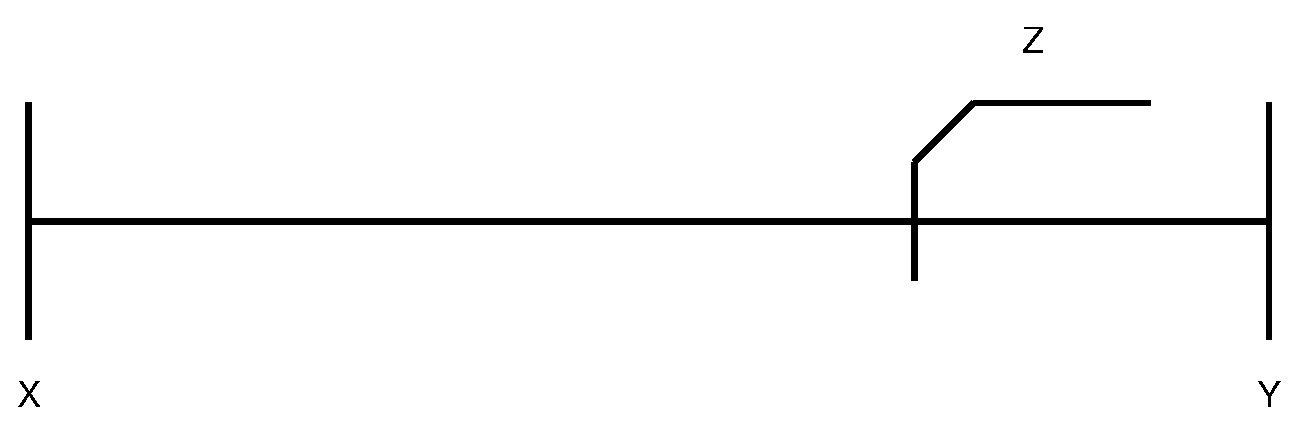
\includegraphics[scale=0.5]{\rootpath/worksheets/evaluation/figures/eval_example}
\caption{Example of characteristic evaluation scale}\label{fig:evel_example}
\end{figure}
Giving each concurrency approach a visual placement allows for improved communication of the findings along with the ability to easily compare the placement of each concurrency approach.

\section{Implementations}
To ensure common ground between all implementations of a particular problem, a set of requirements detailing common factors which must be true for all implementations of a particular problem has been created.

The Dining Philosophers implementations must:
\begin{itemize}
	\item Encompass two 100 milliseconds thread sleeps. One to exemplify the act of eating as well as one upon completing an attempt to eat exemplifying sleeping a period before attempting to eat again.
\end{itemize}

The santa claus problem implementations must:
\begin{itemize}
	\item Follow the requirements defined in \cite{trono1994new}
	\item Utilize advantageous features of the concurrency approach.
\end{itemize}

The concurrent hashmap implementations must:
\begin{itemize}
	\item Encompass fined grained synchronization, allowing multiple threads to operate on the hashmap simultaneously.
\end{itemize}
The implementations in their full length can be found in the appendix.\toby{indsæt et reference når de indsætts}

\section{Evaluation of Characteristics}
All of the selected concurrency approaches relies on starting threads in order to introduce concurrency as well as manually specifying critical regions using ether locks or the \bscode{atomic} block. 
\subsection{Implicit or Explicit Concurrency}
The two \ac{STM} based approaches have implicit elements\toby{Ved ikke om man kan sige det med elements? Måske brug features istedet, eller formuler det til at det det er mere implicit eller mere mod den implicitte ende? (elements udtrykket er brugt i næste subsektion også)} as \ac{STM} allows them to hide the details synchronization. Locking in C\# on the other hand requires explicit stating how synchronization is to be achieved. As such we say that locking in C\# resides close to the explicit concurrency extreme\toby{har vi en grund til at den ikke ligger på explicit? - vil Lone nok spørge} while \stmnamesp and the \ac{STM} library resides slightly more towards the implicit concurrency end of the spectrum. The placement of the three concurrency approaches on the implicit - explicit concurrency spectrum is depicted in \bsref{fig:char_implicit_explicit}.

\begin{figure}[htbp]
\centering
 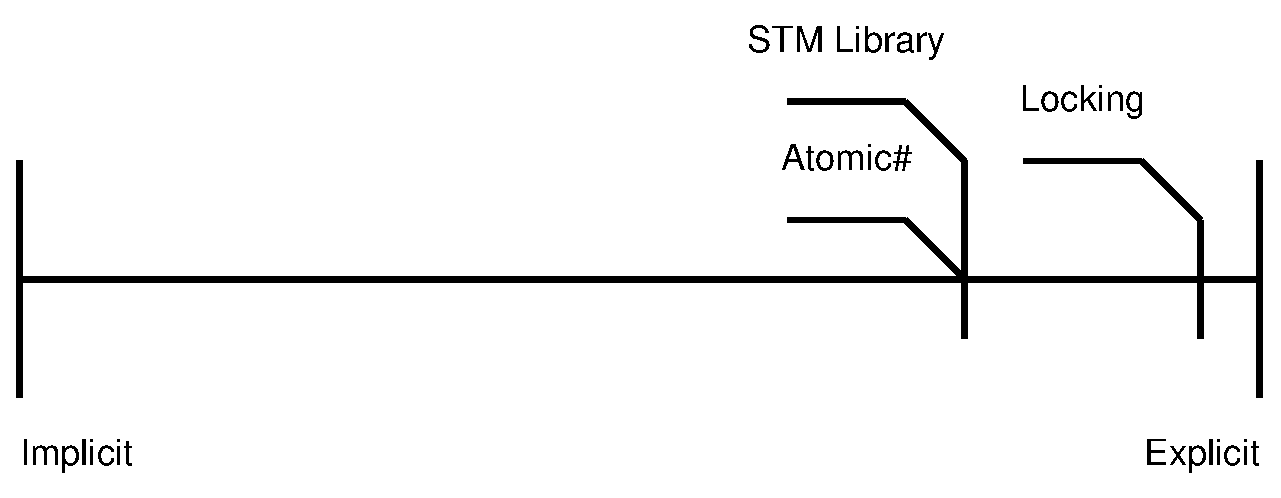
\includegraphics[width=0.9\textwidth]{\rootpath/worksheets/evaluation/figures/char_implicit_explicit} 
 \caption{Concurrency approaches on the implicit - explicit concurrency spectrum}
\label{fig:char_implicit_explicit}
\end{figure}

\subsection{Fault Restrictive or Expressive}
Locking presents the programmer with a set of tools aimed at solving concurrency problems but does little to guarantee their correct usage. Locking in C\# provides the \bscode{lock} statement\cite[p. 102]{csharp2013specificaiton}, which defines a scope within which a given lock is held. The \bscode{lock} statement handles lock acquisition and release which removes the threat of programmers unintentionally missing to release an acquired lock. The lock statement is however only applicable in some scenarios and does, for example, not support timeouts on lock acquisition. As such, we say that locking in C\# resides at the expressive end of the spectrum.

The \ac{STM} based approaches delegate the details of how synchronization is achieved to the underling \ac{STM} system, allowing \ac{STM} based concurrency to avoid some of the errors associated with locking, such as deadlocks. The \ac{STM} based approaches however still rely on shared memory for communication and require programmers to define transaction scopes and introduce concurrency by starting threads. As such the \ac{STM} based approaches reside towards the expressive end of the spectrum but contain elements of fault restrictions pulling it more towards the fault restrictive extreme than locking. The placement of the three concurrency approaches on the fault restrictive - expressive spectrum is depicted in  \bsref{fig:char_fault_expressive}. 
\begin{figure}[htbp]
\centering
 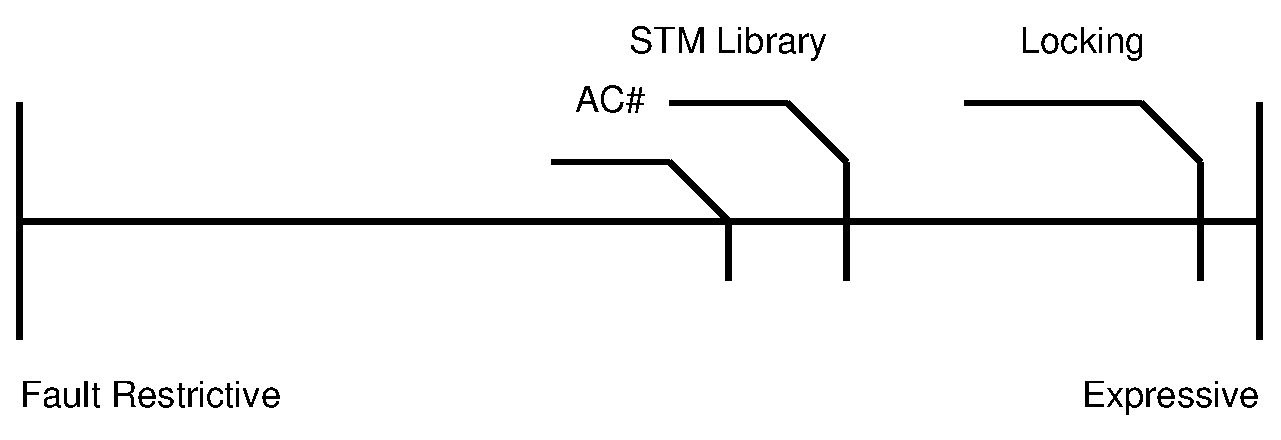
\includegraphics[width=0.9\textwidth]{\rootpath/worksheets/evaluation/figures/char_fault_expressive} 
 \caption{Concurrency approaches on the fault restrictive - expressive spectrum}
\label{fig:char_fault_expressive}
\end{figure}

\subsection{Pessimistic or Optimistic}
Locking assumes that errors are common and therefore allows only a single thread to access a given critical region at a time, by enforcing mutual exclusion. As such locking is an inherently pessimistic concurrency approach. \ac{STM} on the other hand allows multiple threads to proceed simultaneously, correcting any errors that may occur by aborting and re-executing transactions. Hence \ac{STM} takes an optimistic approach to concurrency.
Therefore we say that \stmnamesp and the \ac{STM} library resides at the optimistic extreme of the pessimistic - optimistic spectrum while locking resides at the pessimistic extreme. The placement of the three concurrency approaches on the fault restrictive - expressive spectrum is depicted in \bsref{fig:char_pes_opti}. 
\begin{figure}[htbp]
\centering
 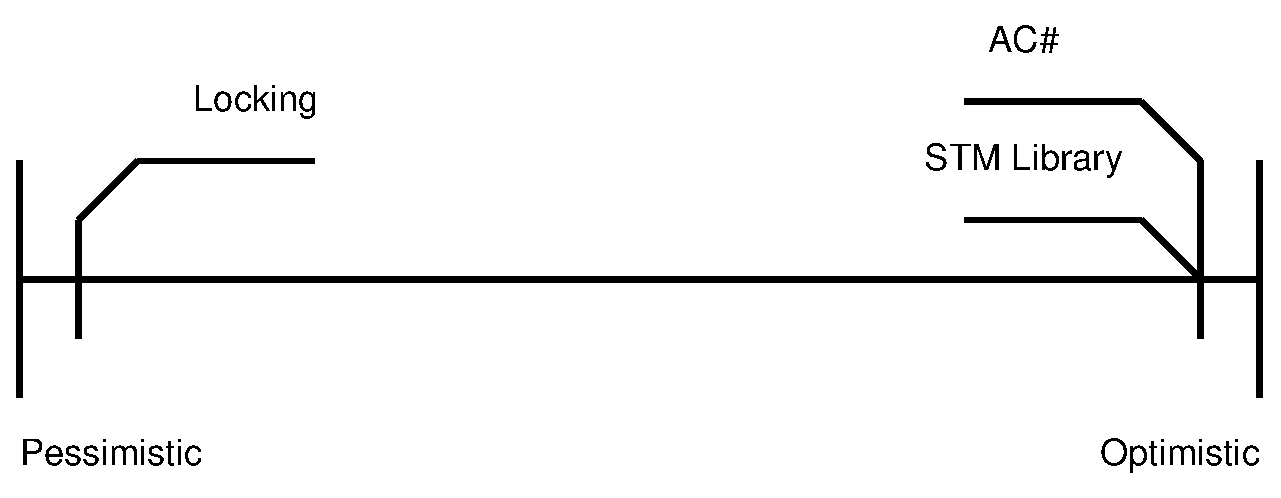
\includegraphics[width=0.9\textwidth]{\rootpath/worksheets/evaluation/figures/char_pessimistic_optemistic} 
 \caption{Concurrency approaches on the pessimistic - optimistic spectrum}
\label{fig:char_pes_opti}
\end{figure}

\subsection{Readability \& Writability}\label{subsec:tl_charac_read_and_write}
The evaluation of readability and writability are based on a number of shared criteria: Simplicity, Orthogonality, Data Types, and Syntax Design. The last two come in addition to the criteria used in the evaluation model defined in our prior work\cite[p. 16-21]{dpt907e14trending}. The reason being, that it is now a concurrency approach in a language, and not the isolated concurrency model. The analysis of Data Types and Syntax Design will not be evaluated on a spectrum of two extremes, as the choices made are trade offs affecting other characteristics, e.g. simplicity and readability. The analysis will therefore be taken into account when the other characteristics is evaluated.

In addition to the shared criteria, writability is based on the level of abstraction and expressivity.
%that of simplicity and orthogonality as well as a number of other considerations. Simplicity and orthogonality is described in the following sections followed by a final evaluation of readability.
\subsubsection{Data Types}\label{subsec:datatypes}\toby{Flyt den ned under syntax design (giver vel mere mening)}
All the concurrency approaches is either integrated or build around C\#, which means that they largely have the same data types. However a transactional variables are treated differently in each \ac{STM} approach. In library \ac{STM}, transactional variables are defined using transactional types, such as \bscode{TMInt}, which means that it is possible to create an array or list containing these types, e.g. \bscode{TMInt[]} defines an array of \bscode{TMInt} types. In \stmname it does not treat transactional variables as transactional types, but instead as regular types with associated \bscode{atomic} keyword modifiers\toby{Hvad type modifer er det præcist?} e.g. \bscode{atomic int}. The result is that it is not possible to define a list or array of transactional variables directly, instead a wrapper class with an \bscode{atomic} field must be employed.

The need to define an array of transactional types was experienced in the hashmap implementations, which uses such an array to represent the buckets of the hashmap. \bsref{lst:lib_Buckets} and \bsref{lst:lang_Buckets} shows how the hashmap buckets are defined in the \ac{STM} library and \stmname, respectively. In the library \ac{STM} example on line \ref{lst:lib_Buckets} the buckets are defined directly. The type of the \bscode{\_buckets} field will be explained gradually. The inner \bscode{Node} type, is a simple class which represents a key value pair, where the value is a transactional variable, defined in the \ac{STM} library code on line \ref{line:lib_node_c} and in \stmname code on line \ref{line:lang_node_c}. The \bscode{Node} is wrapped in an \bscode{ImmutableList} which represents the collision list of a given bucket. The list is immutable for the \ac{STM} system to be able to track changes to the list, as the tracking granularity is only on variables, as described in \bsref{sec:tracking}, and if it was a regular list which changed, the \ac{STM} system would not notice it. The \bscode{ImmutableList} is wrapped in a \bscode{TMVar} for the \ac{STM} system to track changes to the list, each of these then represent a single bucket which is why there is an array of these types. Finally this array is also wrapped in a \bscode{TMVar} allowing the \ac{STM} system to track assignments to the entire backing array in order to resize it when it reaches the load factor threshold. In the \stmname example on line \ref{line:lang_bucket} it is not possible to define the array of transactional variables directly, so a wrapper type called \bscode{Bucket} defined on line \ref{line:lang_bucket_class} is used.

\begin{lstlisting}[float,label=lst:lib_Buckets,
  caption={HashMap Buckets Array - \ac{STM} Library},
  language=Java,  
  showspaces=false,
  showtabs=false,
  breaklines=true,
  showstringspaces=false,
  breakatwhitespace=true,
  escapechar=~,
  commentstyle=\color{greencomments},
  keywordstyle=\color{bluekeywords},
  stringstyle=\color{redstrings},
  morekeywords={atomic, retry, orelse, var, get, set, ref, out}]  % Start your code-block
  
  public class StmHashMap<K,V> : BaseHashMap<K,V>
  {
    //TMVar to (array of TMVars to (ImmutableList of nodes) )
    private readonly TMVar<TMVar<ImmutableList<Node>>[]> _buckets =~\label{line:lib_bucket}~
    new TMVar<TMVar<ImmutableList<Node>>[]>();
  
    ...  //Other code
  
    private class Node~\label{line:lib_node_c}~
    {
      public K Key { get; private set; }
      public TMVar<V> Value { get; private set; }
      public Node(K key, V value)
      {
        Key = key;
        Value = new TMVar<V>(value);
      }
    }
  }
\end{lstlisting}

\begin{lstlisting}[float,label=lst:lang_Buckets,
  caption={HashMap Buckets Array - \stmname},
  language=Java,  
  showspaces=false,
  showtabs=false,
  breaklines=true,
  showstringspaces=false,
  breakatwhitespace=true,
  escapechar=~,
  commentstyle=\color{greencomments},
  keywordstyle=\color{bluekeywords},
  stringstyle=\color{redstrings},
  morekeywords={atomic, retry, orelse, var, get, set, ref, out}]  % Start your code-block
  
  public class StmHashMap<K,V> : BaseHashMap<K,V>
  {
    private atomic Bucket[] _buckets;~\label{line:lang_bucket}~
  
    ... //Other code
    
    private class Bucket~\label{line:lang_bucket_class}~
    {
      public atomic ImmutableList<Node> Value { get; set; }
      public Bucket()
      {
        Value = ImmutableList.Create<Node>();
      }
    }
  
    private class Node ~\label{line:lang_node_c}~
    {
      public K Key { get; private set; }
      public atomic V Value { get; set; }
      public Node(K key, V value)
      {
        Key = key;
        Value = value;
      }
    }
  }
\end{lstlisting}

Ultimately prohibiting the programmer to define an array or list of transactional types directly, lowers the readability and writability\toby{Skal vi anvende andre karaktirisikter den påvirker negativt? Hvad expressivity før, men den er påvirker kun writability} of \stmname, as it is requires the programmer to write, read and maintain this extra wrapper code.\toby{Evt. noget med at det er en følge af design valg (ingen silver bullet)}

%Extra der påvirker data types:
	%Måske nævn det har samme behaviour som virtual modifieren (var det ikke det du sagde kasper?)
	%Måske noget om at ac# fungerer også med ref og out (som library ikke kan), så det har en bedre integartion med datatyperne i sporget?? (men det er jo keywords det integreres med, så måske en anden formulering)
	%Andreas skrevet: Using STM types could imply a different meaning and confusing the programmer. Is TMInt the same value as int?
\subsubsection{Syntax Design}\label{subsec:syntaxdesign}
\andreas[inline]{We must explain why we do not use a spectrum}
The use of keywords reduces simplicity but increases readability, as the intent stands out clearly\cite[p. 12-13]{sebestaProLang}. Locking in C\# uses only a single keyword, \bscode{lock}. The rest of the functionality is provided by library calls as described in \andreas{REF til hvor det ender med at stå}. The use of libraries for locking constructs makes it blend in with other library code, even though it got a special purpose. This decreases the readability, but keeps the simplicity of the language high as it does not introduce keywords for all constructs. 

The \ac{STM} library also uses library calls just as described above, thus it got the same disadvantages and the readability is decreased compared to \stmname which got keywords for the special constructs. The four keywords introduces in \stmname does however decreases the simplicity of the language. As the \bscode{atomic} keyword got different meanings depending on the context in \stmname, its readability is lowered and the simplicity is raised by keeping a minimum of keywords. 

In \stmname, an \bscode{atomic} variable can be passed directly as a non-\bscode{atomic} argument, and the language will provide the encapsulated value. In the \ac{STM} library, this is not the case, and the programmer has to manually call the \bscode{Value} property on the \bscode{atomic} variable to get the value. In this case, both the readability and simplicity is increased in \stmname compared to the \ac{STM} library, as the code gets less cluttered, thus easier to read.

In C\# it is possible to name variables by reserved keywords, by prefixing the name with \bscode{@}. Due to this, the additional keywords in \stmname does not restrict the use of variable naming, and it clearly distinguish when it is used as a name or a keyword.

\subsubsection{Low or High Simplicity}\label{subsec:simplicity}
Locking is based on the idea of mutual exclusion. C\# supplies a number of different constructs, with slight variations, for defining synchronization using locking. Applying locking correctly in complex scenarios is considered to be hard\cite[p. 56]{sutter2005software}. Mainly due to the number of errors that can arise, such as deadlocks. 

Locking requires the programmer to explicitly state how synchronization is to be applied. Both library based \ac{STM} and \stmname take a more declarative approach than locking when specifying what needs to be synchronized, thus it is simpler as the programmer does not have to worry about the lower level details.\andreas{Skal vi have usability study ind igen?}\toby{Jaaaaaaaaaa!} In the case where conditional synchronization is needed, both forms of \ac{STM} can leverage the \bscode{retry} functionality and make a transaction block until the variables previously read by the transaction are changed by another transaction. In C\# a \bscode{Monitor} enables waiting until a lock has been freed, but contrary to \bscode{retry} this is not on a declarative level. This is shown in the ConcurrentHashMap example in \bsref{llst:lock_add_hashmap} and \bsref{lst:lang_add_hashmap}, where the need for different locks for different critical regions is clearly displayed. In \bsref{lst:lock_add_hashmap} on line \ref{line:lock_lock_bucket}, a calculation is made to check which needs to be used, additionally on line \ref{line:lock_lock_size} another lock is needed for another critical region. This is entirely avoided in \bsref{lst:lang_add_hashmap} where the entire method is wrapped in an \bscode{atomic} block, and the \ac{STM} system detects and resolves potential conflicts.

Library based \ac{STM} uses existing language constructs, such as static method calls, however it does have not support for checking implicit dependency between static calls at compile time, e.g. \bscode{retry} outside an \bscode{atomic} call will not produce a compile time warning. Additionally, the \ac{STM} types provided must be used to track variables in transactions. These types cause a type mismatch when used together with standard types, thus making the library more complex to use. This issue is partly resolved by providing implicit type conversion on the \ac{STM} types, but the implicit conversion is not possible in all cases. In the cases where it is not, the programmer must access the non-\ac{STM} type by the \bscode{Value} property available on all \ac{STM} types. 

\stmnamesp introduces additional language constructs which reduces the simplicity of the language. It does however increase the simplicity of using the \ac{STM} part, e.g. using \bscode{retry} outside of an \bscode{atomic} block will result in a compile time warning. Additionally, \bscode{atomic} can also be used to modify fields, local variables and parameters, making them traceable in transactions without having to use specific types. This simplifies interaction between code that uses \bscode{atomic} variables and code that does not. 

\begin{lstlisting}[float,label=lst:lock_add_hashmap,
  caption={ConcurrentHashMap \bscode{Add} Method - Locking},
  language=Java,  
  showspaces=false,
  showtabs=false,
  breaklines=true,
  showstringspaces=false,
  breakatwhitespace=true,
  escapechar=~,
  commentstyle=\color{greencomments},
  keywordstyle=\color{bluekeywords},
  stringstyle=\color{redstrings},
  morekeywords={atomic, retry, orelse, var, get, set, ref, out}]  % Start your code-block

  public override void Add(K key, V value)
  {
      var hashCode = GetHashCode(key);
      lock (_locks[GetLockIndex(hashCode)])~\label{line:lock_lock_bucket}~
      {
          var bucket = _buckets[GetBucketIndex(hashCode)];
          var node = FindNode(bucket, key);

          if (node != null)
          {
              //If node is not null, key exist in map. Update the value
              node.Value = value;
          }
          else
          {
              //Else insert the node
              bucket.AddFirst(CreateNode(key, value));
              lock (_sizeLock)~\label{line:lock_lock_size}~
              {
                  _size++;
              }
              ResizeIfNeeded();
          }
      }
  }
\end{lstlisting}

\begin{lstlisting}[float,label=lst:lang_add_hashmap,
  caption={ConcurrentHashMap \bscode{Add} Method - \stmname},
  language=Java,  
  showspaces=false,
  showtabs=false,
  breaklines=true,
  showstringspaces=false,
  breakatwhitespace=true,
  escapechar=~,
  commentstyle=\color{greencomments},
  keywordstyle=\color{bluekeywords},
  stringstyle=\color{redstrings},
  morekeywords={atomic, retry, orelse, var, get, set, ref, out}]  % Start your code-block
  
  public override void Add(K key, V value)
  {
      atomic
      {
          var bucketIndex = GetBucketIndex(key);
          //TMVar wrapping the immutable chain list
          var bucketVar = _buckets[bucketIndex];
          var node = FindNode(key, bucketVar.Value);
         
          if (node != null)
          {
              //If node is not null key exist in map. Update the value
              node.Value = value;
          }
          else
          {
              //Else insert the node
              bucketVar.Value = bucketVar.Value.Add(CreateNode(key, value));
              _size++;
              ResizeIfNeeded();
          }
      }
  }
\end{lstlisting}

The placement of the three concurrency approaches on the low simplicity - high simplicity spectrum is depicted in \bsref{fig:char_simplicity}.

\begin{figure}[htbp]
\centering
 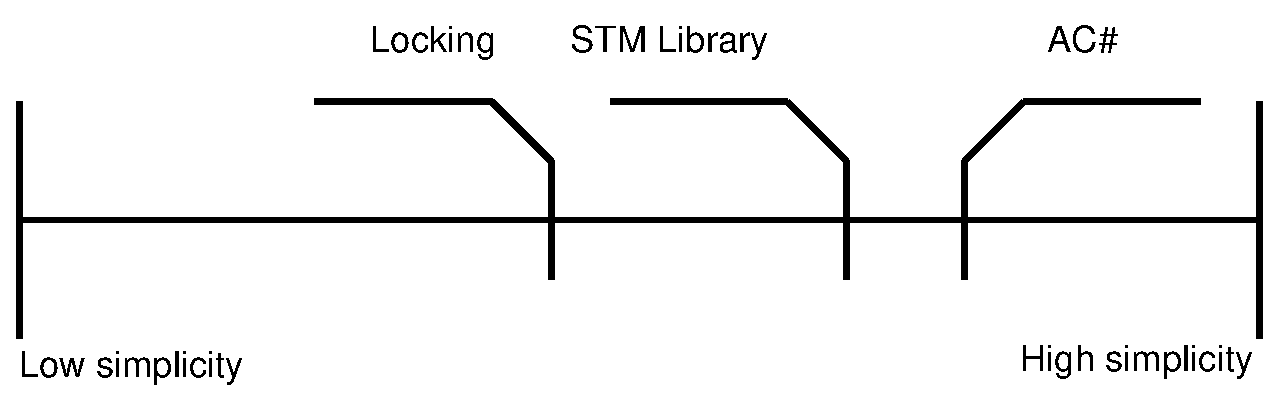
\includegraphics[width=0.9\textwidth]{\rootpath/worksheets/evaluation/figures/char_read_simplicity} 
 \caption{Concurrency approaches on the low - high simplicity spectrum}
\label{fig:char_simplicity}
\end{figure}
% Additional constructs: Atomic block, orelse, retry, atomic fields
% In language atomic is a modifier, not a type (atomic int can be passed into an int param)	. The .value can be skipped. 
% Conditional syncronization is very easy in STM
% Waiting on a certain key on a hashmap is hard to implement with locks, but easy with STM.
% Concurrency related issues are fewer in STM
\subsubsection{Low or High Orthogonality}\label{subsec:orthogonality}
Locking encompasses a number of basic constructs aimed at aiding in different concurrency scenarios. These constructs can be combined to handle complex concurrency issues. Some of these combinations are however erroneous producing hard to debug problems such as deadlocks. Locking does not put any restraints on the language features with which it can be combined and may therefore seam to be highly orthogonal. The threat of deadlocks when combining lock based implementations or employing multiple locks limits the orthogonality keeping locking from reaching the high orthogonality extreme. Locking in C\# provides no solutions to these issues. As a result we say that locking in C\# resides just above the middle of the spectrum towards the high orthogonality end of the spectrum.

\ac{STM} removes the issue of deadlocks and allows \ac{STM} based code segments to be combined using transactional nesting. \ac{STM} however combines poorly with irreversible actions, that is actions which can not be rolled back in case a transaction aborts such as \ac{IO}. Neither the \ac{STM} library nor \stmnamesp offers a solution to this problem reducing their orthogonality. 

The \ac{STM} library uses special types for transactional variables, which requires the programmer to use the \bscode{Value} property whenever they need to make an assignment. Implicit conversion ensures that an object of one of the \ac{STM} types, such as \bscode{TMInt}, can, in most cases, be used as if it was an object of the type its wrapping. \bsref{lst:lib_implicit_conversion} shows an equality comparison of two transactional variables using the \ac{STM} library. The comparison on line \ref{line:lib_equality} requires the programmer to access the \bscode{Value} property of the \bscode{TMVar} objects as implicit conversion will not be used if the \bscode{TMVar}'s are compared directly, resulting in reference comparison of the \bscode{TMVar} objects producing an incorrect result. A similar problem exists when calling a method on a \bscode{TMVar} object, implicit conversion does not allow methods of the wrapped type to be called on the \bscode{TMVar} directly. Such cases reduce the orthogonality of the \ac{STM} library. The \ac{STM} library however still benefits from the advantages provided by \ac{STM} and is placed just to the right of locking on the low - high orthogonality spectrum.

\begin{lstlisting}[label=lst:lib_implicit_conversion,
  caption={Equality comparison of \bscode{TMVar<bool>}},
  language=Java,  
  showspaces=false,
  showtabs=false,
  breaklines=true,
  showstringspaces=false,
  breakatwhitespace=true,
  escapechar=~,
  commentstyle=\color{greencomments},
  keywordstyle=\color{bluekeywords},
  stringstyle=\color{redstrings},
  morekeywords={atomic, retry, orelse, var, get, set, ref, out, bool}]  % Start your code-block

  public bool TestMethod()
  {
    TMVar<bool> v1 = new TMVar<bool>(false);
    TMVar<bool> v2 = new TMVar<bool>(false);
    return v1.Value == v2.Value;~\label{line:lib_equality}~
  }
\end{lstlisting}
\stmnamesp treats transactional variables as an object of their original type, allowing the programmer to compare the value directly. Methods can be invoked directly on the transactional variable, without having to reason about implicit conversion or manually accessing the \bscode{Value} property, as described above. Therefore \stmname is placed more towards the high orthogonality end of the spectrum than the other two approaches. 

The placement of the three concurrency approaches on the low - high orthogonality spectrum is depicted in \bsref{fig:char_orthogonality}.


%orthogonality
%locking deadlocks
%types in language
%++ -- operators
%STM, IO
\begin{figure}[htbp]
\centering
 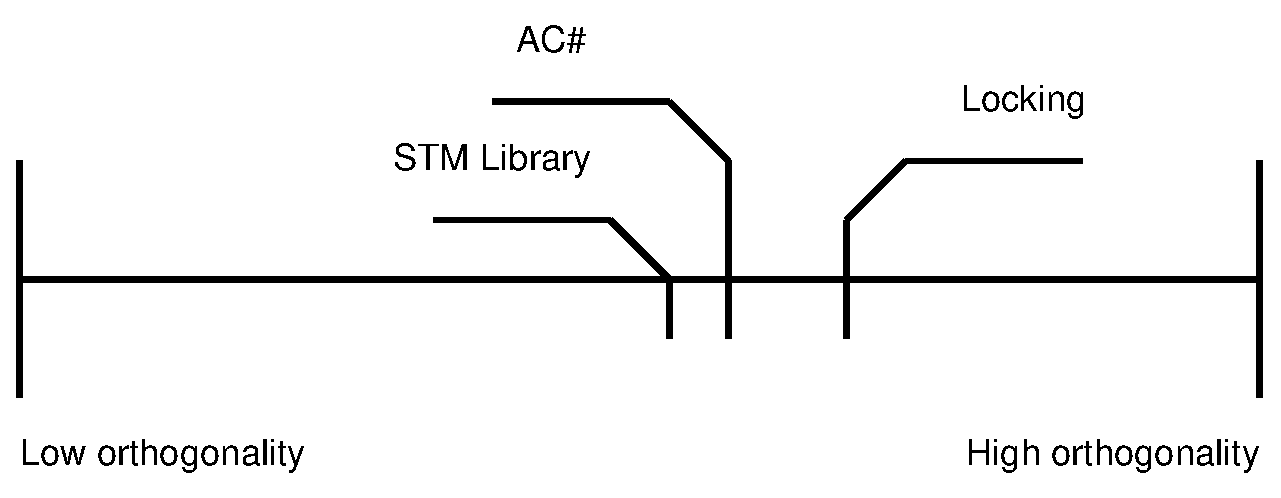
\includegraphics[width=0.9\textwidth]{\rootpath/worksheets/evaluation/figures/char_orthogonality} 
 \caption{concurrency approaches on the low - high orthogonality spectrum}
\label{fig:char_orthogonality}
\end{figure}

\subsubsection{Low or High Readability}\label{subsec:char_readability}
As described in \bsref{subsec:syntaxdesign} the syntax design of locking BLA\toby{Something about the syntax design on each model}. In \bsref{subsec:simplicity} the simplicity of locking is placed close to the low simplicity extreme, where the \ac{STM} library is placed a bit higher than the middle of the spectrum and \stmname even higher. In \bsref{subsec:orthogonality} the orthogonality of locking resides just above the middle of the spectrum, where the \ac{STM} library resides a little higher and \stmname again a little higher. These characteristics directly influence the readability of the concurrency approaches.\toby{Evt. flyt disse referencer ned under den enkelte approach og vær med uddybende. Hvis ikke det gøres skal der også en reference til data types section}

All the concurrency approaches have to explicitly mark critical regions of code in order to ensure a program is race condition free. This negatively affects the readability of all the approaches, as by reading the program it is hard to know whether critical regions are marked correctly everywhere, and it is especially hard in large programs.

The basic \bscode{lock} construct and idea behind locking is simple, as simply a resource is locked, preventing others from using it. This positively affects the readability of locking and in small code segments it may seem highly readable. However locking suffers in particular from the concurrency issue of deadlocks. This negatively affects the readability of locking, as in order to reason about deadlocks, the programmer has to reason about every code segment where locking is applied and how these segments interact. As locking code can be very fragmented it can become very hard for the programmer to reason about. Additionally, if a program makes use of other libraries that uses locking internally, the programmer also have to reason about the locks contained within those libraries, as locks do not compose. The readability of locking is therefore placed towards low readability on the spectrum.\toby{evt. ref til study om locking er hard, (eller refer til simplicity characterisics hvor det står i}

The \ac{STM} approaches removes the issue of deadlocks, which positively affects the readability, as the programmer does not have to reason about deadlocks. Additionally, \ac{STM} also removes the issue of composing code segments which are marked for synchronization, as \ac{STM} allows for nested transactions. However \ac{STM} suffers from code fragmentation which can make it hard to get an overview of all the \ac{STM} synchronization in a program, which affects the readability negatively. Furthermore understanding the idea behind \ac{STM} can at first be hard to grasp\toby{evt. ref til study}, as it promotes a new way of synchronizing programs, and especially since both the \bscode{orelse} and \bscode{retry} constructs have been included in the \ac{STM} library and \stmname.
%transactions does not work with irreversible actions - kan man sige noget om det i forhold til readability?
	%nok mere writability

%problematic to predict the performance of transactions (skal vi have det med?)

\toby[i]{Fortæl om stm lib og \stmname individuelt - brug data typer og syntax design til at vælge placeringer mellem dem)}

The placement of the three concurrency approaches on the low readability - high readability spectrum is shown in \bsref{fig:char_readability}.

\begin{figure}[htbp]
\centering
 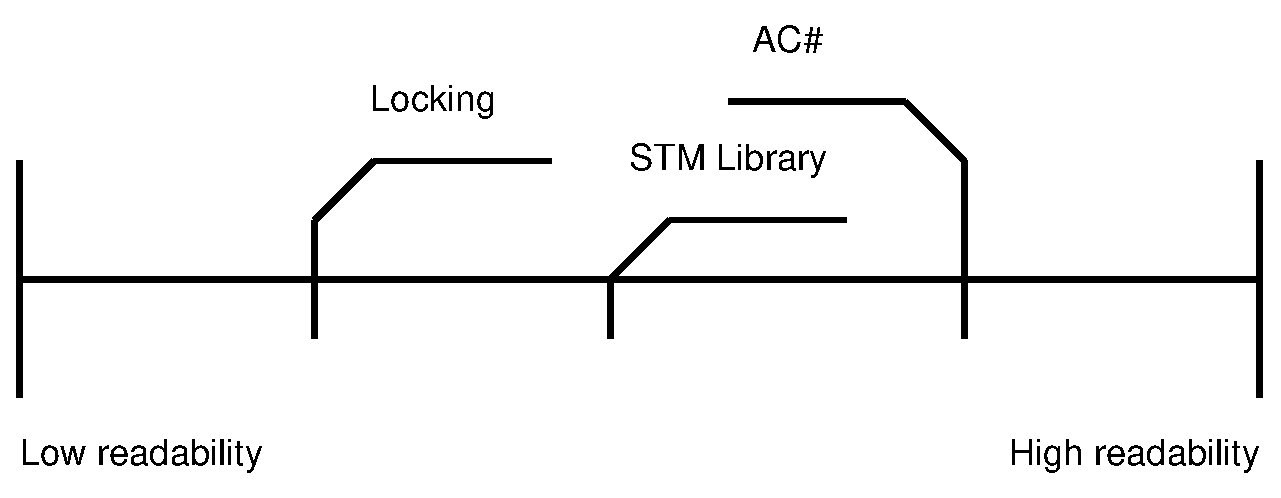
\includegraphics[width=0.9\textwidth]{\rootpath/worksheets/evaluation/figures/char_readability} 
 \caption{Concurrency approaches on the low - high readability spectrum}
\label{fig:char_readability}
\end{figure}

\subsubsection{Low or High Level of Abstraction}\label{subsec:level_of_abstraction}
Locking is tightly coupled with the hardware architecture through hardware instructions such as Test-and-set and Compare-and-swap\cite[p. 1990]{scott2011sync}. Furthermore low-level abstraction threads are used in order to introduce concurrency. Additionally the programmer has to state exactly how synchronization should be applied using locks. C\# offers the lock \bscode{lock} statement which provides a small abstraction over the release of a lock. The \bscode{lock} statement is however not applicable in all cases. If for example a timeout on the acquisition of a lock is required or a more advanced form of lock, such as a semaphore, is required, the \bscode{lock} keyword is not directly applicable. This can also been seen in the implementations for the evaluation. Both the locking Dining Philosophers implementation and the lock based concurrency hashmap implementation require the use of the monitor class instead of the lock keyword for acquiring a lock with a timeout. The Dining Philosophers implementation requires the second lock to be taken with a timeout and the concurrency hashmap implementation uses a timeout with acquiring the lock on resizing the backing array\lone{Forklar hashmap impl}. Furthermore the flow of the locking Santa Claus implementation uses semaphores to signal between santa, the elfs and the reindeer. The \bscode{lock} keyword does not provide such capabilities. Ultimately locking in C\# is placed close to the low level of abstraction extreme of the spectrum with the small abstractions provided keeping it from being at the extreme. 

The \ac{STM} approaches also rely on threads, but provide a higher level of abstraction for synchronization. \ac{STM} uses transactions, where code segments are marked and the details of how synchronization is achieved is abstracted away to the \ac{STM} system. However the isolation level can pose a threat to the level of abstraction of transactions, as under weak isolation \ac{STM} will not take non-transactional code into account and the programmer must therefore manage it. In the case of \stmnamesp this is not problematic, as it facilities strong atomicity, as described in \bsref{sec:design_strong_weak_atomicity} and the \ac{STM} system will therefore manage both transactional and non-transactional code. Based on the above, the general \ac{STM} approach lies between the middle and high end of the spectrum, where the main negative factors is that the programmer still has to manage threads and mark regions of code that should be synchronized.

As to the language \ac{STM} and library \ac{STM} individually, some differences in the level of abstraction exist. Library \ac{STM} requires the programmer to use static method calls, wrap transactional code in lambdas, wrap transactional variables in a \bscode{TMVar}, use the \bscode{Value} property when getting or setting a value, supply \bscode{orelse} transactions as arguments to the atomic method call, and write return in front of the static method call if a method must return the value computed by a transaction. Many of these concerns are abstracted away or handled more gracefully in the language based \ac{STM}. \bsref{lst:lib_SleepUntilAwoken} and \bsref{lst:lang_SleepUntilAwoken} present an implementation of the \bscode{SleepUntilAwoken} method from the library and language based Santa Claus problem implementations, respectively. The method ensures that santa sleeps until he is awoken by either three elfs at his door, or all reindeers back from vacation ready to fly his sleigh. The \bscode{return} statement on line \ref{line:lib_sleep_return} of \bsref{lst:lib_SleepUntilAwoken} is not present in the language based implementation as it is abstracted away by \stmnamesp. Furthermore the static method call and creation of lambas to represent transaction bodies on line \ref{line:lib_sleep_return} is abstracted away by the \bscode{atomic} block and orelse block on lines \ref{line:lang_sleep_atomic} and \ref{line:lang_sleep_orelse} of \bsref{lst:lang_SleepUntilAwoken}.

\begin{lstlisting}[float,label=lst:lib_SleepUntilAwoken,
  caption={\bscode{SleepUntilAwoken} Method - \ac{STM} Library},
  language=Java,  
  showspaces=false,
  showtabs=false,
  breaklines=true,
  showstringspaces=false,
  breakatwhitespace=true,
  escapechar=~,
  commentstyle=\color{greencomments},
  keywordstyle=\color{bluekeywords},
  stringstyle=\color{redstrings},
  morekeywords={atomic, retry, orelse, var, get, set, ref, out}]  % Start your code-block

  private WakeState SleepUntilAwoken()
  {
    return STMSystem.Atomic(() =>~\label{line:lib_sleep_return}~
    {
      if (_rBuffer.Count != SCStats.NR_REINDEER)
      {
        STMSystem.Retry();
      }
      return WakeState.ReindeerBack;
    },
      () =>~\label{line:lib_t2_def}~
      {
        if (_eBuffer.Count != SCStats.MAX_ELFS)
        {
          STMSystem.Retry();
        }
        return WakeState.ElfsIncompetent;
      });
  }
\end{lstlisting}

\begin{lstlisting}[float,label=lst:lang_SleepUntilAwoken,
  caption={\bscode{SleepUntilAwoken} Method - \ac{STM} Language},
  language=Java,  
  showspaces=false,
  showtabs=false,
  breaklines=true,
  showstringspaces=false,
  breakatwhitespace=true,
  escapechar=~,
  commentstyle=\color{greencomments},
  keywordstyle=\color{bluekeywords},
  stringstyle=\color{redstrings},
  morekeywords={atomic, retry, orelse, var, get, set, ref, out}]  % Start your code-block

  private WakeState SleepUntilAwoken()
  {
    atomic~\label{line:lang_sleep_atomic}~
    {
      if (_rBuffer.Count != SantaClausProblem.NR_REINDEER)
      {
        retry;
      }
      return WakeState.ReindeerBack;
    }
    orelse~\label{line:lang_sleep_orelse}~
    {
      if (_eBuffer.Count != SantaClausProblem.MAX_ELFS)
      {
        retry;
      }
      return WakeState.ElfsIncompetent;
    }
  }
\end{lstlisting}

Furthermore, where the \ac{STM} library exposes transactional variables as special \ac{STM} types, \stmnamesp instead allows variables to be marked as \bscode{atomic}, letting the programmer use the variable as if it was of the original type, even though the type is changed as part of the compilation process. Language \ac{STM} is therefore considered to have a higher level of abstraction than library \ac{STM}. As described previously \ac{STM} however combines poorly with irreversible actions leaving it up to the programmer to correctly handle actions such as \ac{IO} in combination with transactions. As neither the \ac{STM} library nor \stmnamesp presents a solution to this problem their level of abstraction is reduced.

The placement of the three concurrency approaches on the low level of abstraction - high level of abstraction spectrum is depicted in \bsref{fig:char_level_of_abstraction}. 

\begin{figure}[htbp]
\centering
 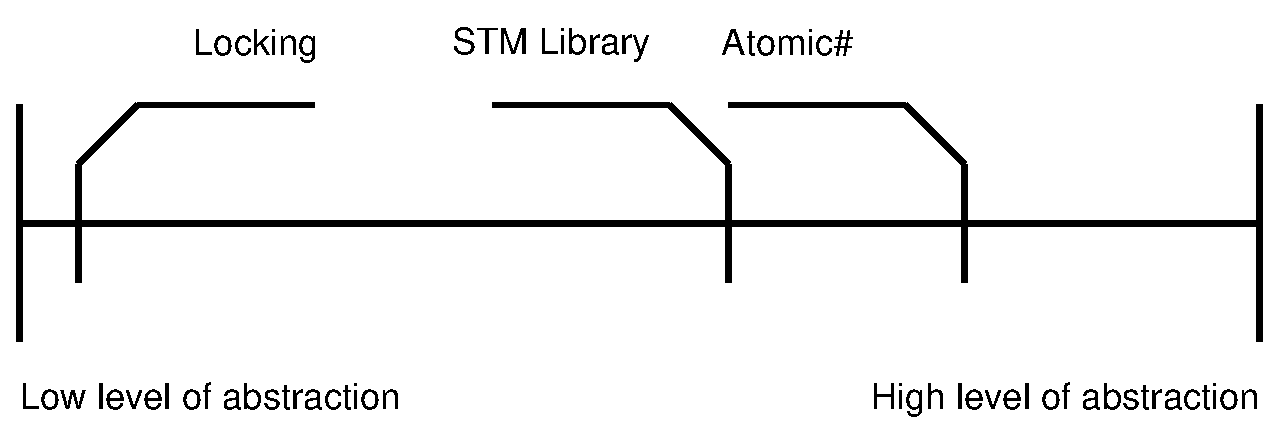
\includegraphics[width=0.9\textwidth]{\rootpath/worksheets/evaluation/figures/char_level_of_abstraction} 
 \caption{Concurrency approaches on the low - high level of abstraction spectrum}
\label{fig:char_level_of_abstraction}
\end{figure}

\subsubsection{Low or High Expressivity}\label{subsec:expressivity}
%The expressivity of the approaches are closely related to their level of abstraction. 
Locking in C\# is mainly accomplished by the use of the \bscode{lock} keyword, which provide a convenient way to acquire and release a lock on a resource, by creating a scope in which the lock is automatically taken in the beginning and released at the end of the scope. However it is not always sufficient, instead the \bscode{Monitor} class can be used which provides additional functionality, such as the \bscode{TryEnter} method. Furthermore, there are a number of other special case locking constructs in C\#\cite{microsoftSyncPrim} i.e. \bscode{Mutex,} \bscode{Semaphore,} \bscode{SpinLock} and \bscode{ReaderWriterLock,} that can help the programmer specify synchronization. These locking constructs enable ways to express exactly how synchronization should be applied by the use of locks and it therefore affects the expressivity positively. The fact that locking uses constructs close to the hardware primitives and that  locking is prone to a number of concurrency related issues, such as deadlocks, causes its expressivity to be reduced. Locking in C\# gives the programmer control over many low level details concerning how synchronization is applied but at the same time requires the programmer to specify these details. This along with the threat of deadlocks and other issues limits how the programmer can concisely and conveniently express the functionality. Locking in C\# is therefore placed towards low expressivity, being drawn a bit towards the middle of the spectrum because of the many convenient locking constructs in C\#.

\ac{STM} also builds upon threads which limits its expressivity. Transactions however represent a more declarative and expressive approach than locking, as the programmer only have to specify critical regions and the \ac{STM} system will then manage exactly how synchronization is applied. This affects the expressivity both positively and negatively, as it accomplishes a great deal of computation with little code, but it also denies the programmer the possibility to express low level synchronization details. Furthermore \ac{STM} eliminates the issues of deadlocks which makes it more convenient to express synchronization, as the programmer does not have to reason about it. However, neither in the \ac{STM} library or \stmname there exists not a convenient way to express irreversible actions, such as exceptions and \ac{IO}, the programmer is left alone in ensuring these actions works correctly with transactions, which negativity affects the expressivity. Based on the above, the general \ac{STM} approach is placed between the middle and high end of the spectrum.

As to \stmname and library \ac{STM}, there are some differences in how expressive the approach is. The expressiveness of the approach is closely related to the level of abstraction of the approach, described in \bsref{subsec:level_of_abstraction}. As described in that section, library \ac{STM} requires the programmer to put extra effort into expressing the intended functionality e.g. wrapping transactional code in lambdas, wrapping transactional variables in \bscode{TMVar} types and using the \bscode{Value} property when getting or setting a value on a transactional variable. That is abstracted away in \stmname which makes it more expressive as such it provides a more convenient and less tedious way of specifying computations. However, the abstraction that \stmname provides, also disallows the programmer to define an array of transactional types directly and instead requires the programmer to use a wrapper class, as described in \bsref{subsec:datatypes}. Based on the above, \stmname is considered to have a higher expressivity than library \ac{STM} because of the higher level of abstraction that it facilitates, however not much, as defining an array or list of transactional types directly is disallowed.

The placement of the three concurrency approaches on the low expressivity - high expressivity spectrum is depicted in \bsref{fig:char_expressivity}. 

%expressivity:
%great deal of computation accomplished with a small program
	%fx. retry
%convenient ways of specifying computations
\begin{figure}[htbp]
\centering
 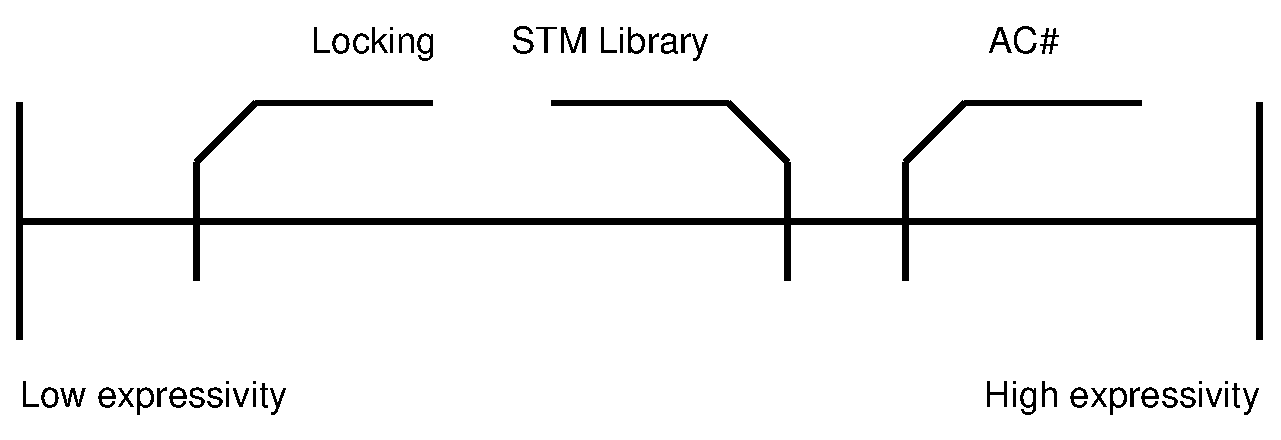
\includegraphics[width=0.9\textwidth]{\rootpath/worksheets/evaluation/figures/char_expressivity} 
 \caption{Concurrency approaches on the low - high expressivity spectrum}
\label{fig:char_expressivity}
\end{figure}

\subsubsection{Low or High Writability}
As discussed in \bsref{subsec:level_of_abstraction} locking in C\# has a low level of abstraction due to its usage of low level constructs. While the \bscode{lock} statement provides a abstraction over the acquisition and release of a lock providing increased writability in cases where it is applicable, the writability of locking in C\# is reduced as a result of the low level of abstraction. The \ac{STM} libraries level of abstraction is said to be be just above the middle towards the high level of abstraction end of the spectrum, while \stmname is said to have a higher level of abstraction than the \ac{STM} library. This positively impacts the writability of the \ac{STM} library and \stmname.

Locking in C\# presents a number of different tools, such as \bscode{Semaphore}'s and \bscode{SpinLock}'s for defining synchronization. These tools are however still prone to common locking problems, such as deadlocks, resulting in a low expressivity score which negatively impacts its writability. The expressivity of the \ac{STM} library resides above the middle of the spectrum. The expressivity of the \ac{STM} library is limited due to the requirements of wrapping transactional code in lambdas, wrapping transactional variables in \bscode{TMVar} types and using the \bscode{Value} property when getting or setting a value on a transactional variable, hindering the programmer in concisely expressing  the intended behavior and resulting in reduced writability. \stmname removes these burdens from the programmer, by delegating them to the compiler, resulting in a higher expressivity score and improved writability.

With respect to simplicity locking in C\# is, as described in \bsref{subsec:simplicity}, placed close to the low simplicity end of the spectrum mainly due the the number of errors that can arise. This negatively impacts the approach's readability. The two \ac{STM} based approaches benefit from \ac{STM} declarative approach to defining synchronization. The \ac{STM} library is placed just above the middle of the spectrum while \stmname resides further towards the high simplicity end of the spectrum. \stmname is given a higher simplicity score due to its cleaner syntax and the ability to use existing types instead of the \ac{STM} equivalents resulting in a greater positive impact on writability.

As described in \bsref{subsec:orthogonality} locking in C\# has properties which seam orthogonal but is limited due to the threat of errors when combining locking constructs. The \ac{STM} based approaches benefit from simplified composition based on transactional nesting but simultaneously introduces issues with irreversible actions such as \ac{IO}. The \ac{STM} library has problems combining with existing types in all cases. Furthermore the implicit conversion feature can not be relied on in all cases, requiring the programmer to access the \bscode{Value} property, reducing the libraries orthogonality. Ultimately this result in the \ac{STM} library being placed just between the middle and the high end of the low - high orthogonality spectrum. \stmname address the issues of the \bscode{STM} library by allowing the programmer to use any existing types instead of the \ac{STM} types and by delegating much of the worked require by the \ac{STM} library to the compiler. This results in \stmname being placed just above the \ac{STM} library on the  low - high orthogonality spectrum. These scores positively impacts the writability of the approaches.

Locking suffers from the fact that a number of serious errors are present resulting in it being hard in complex scenarios limiting its writability. The \ac{STM} based approaches solve many of the errors present with locking but introduces new problems with ireversible actions. Th \ac{STM} library has problems with types, accessing the wrapped value and the syntax of transaction definitions with limits its writability. \stmname addresses many of the writability problems present in the \ac{STM} library by delegating the work to the compiler. Based on these observations and the evaluations of the previous characteristics the three approaches have been placed on the low - high writability spectrum as depicted in \bsref{fig:char_tl_writability}.

\begin{figure}[htbp]
\centering
 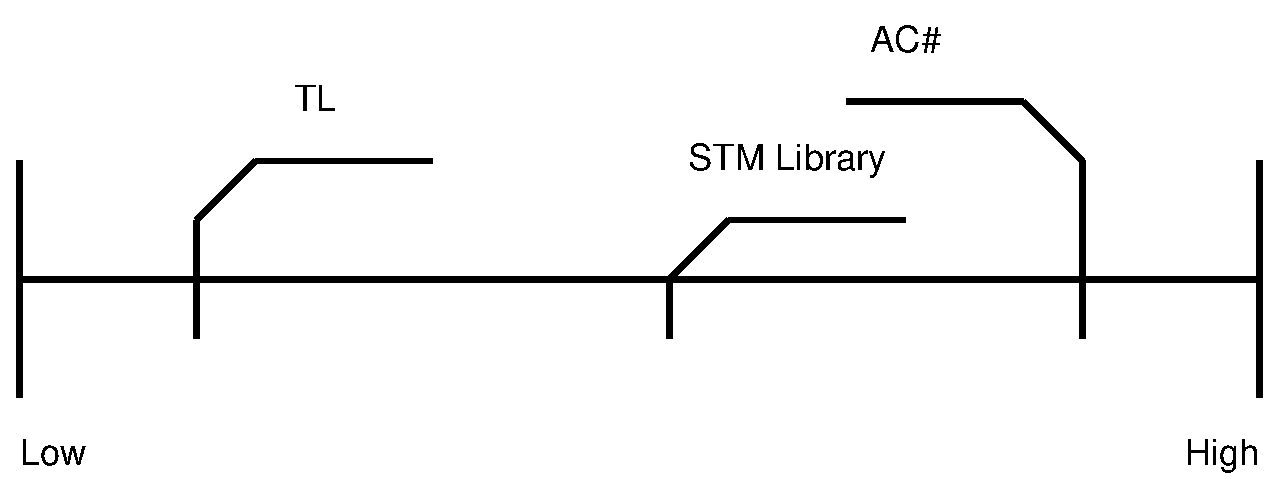
\includegraphics[width=0.9\textwidth]{\rootpath/worksheets/evaluation/figures/char_writability} 
 \caption{Concurrency approaches on the low - high writability spectrum}
\label{fig:char_tl_writability}
\end{figure}

\worksheetend
